\documentclass[conference]{IEEEtran}
\usepackage{cite}
\usepackage{graphicx}
\usepackage[utf8]{inputenc}
\usepackage{multicol}
\usepackage{color} 
\usepackage{setspace}
\usepackage{listings}
\usepackage{wrapfig}
\usepackage[table,xcdraw]{xcolor}
\usepackage{caption}
\usepackage{subcaption}
\usepackage{amsmath}
\usepackage{amssymb}
\usepackage{multirow}
\usepackage{url}
\usepackage{booktabs}
\usepackage{float}
\usepackage{tikz}
\usepackage{pgfplots}
\pgfplotsset{compat=1.18}
\usepgfplotslibrary{groupplots}
\usepgfplotslibrary{polar}
\usetikzlibrary{shapes,arrows,positioning,calc}

\begin{document}

\title{Privacy-Preserving Physiological Signal Classification in Mobile Health: A Comparative Study of Federated Learning and Differential Privacy}

\author{
    \IEEEauthorblockN{
    \textsuperscript{1}Vasco Fernandes,
    \textsuperscript{2}Pedro Martins}
    \IEEEauthorblockA{
    \textsuperscript{1}Department of Informatics, Polytechnic of Viseu, Viseu, Portugal\\
    \textsuperscript{2}Research Center in Digital Services, Polytechnic of Viseu, Viseu, Portugal \\
    \vspace{0.2cm}
    pv25177@alunos.estgv.ipv.pt, pedromom@estgv.ipv.pt}
}

\maketitle

\begin{abstract}
Mobile health (mHealth) applications collect sensitive physiological data from wearable devices, raising significant privacy concerns under regulations such as GDPR. While machine learning models can extract valuable health insights, centralized data processing exposes personal information to potential breaches and unauthorized access. This paper presents a comprehensive experimental evaluation of two privacy-preserving techniques---Federated Learning (FL) and Differential Privacy (DP)---applied to physiological signal classification tasks.

We implement and compare these approaches using two real-world datasets: WESAD (stress detection from 15 subjects) \cite{schmidt2018wesad} and Sleep-EDF (sleep stage classification from approximately 80 subjects) \cite{kemp2000sleep_edf,goldberger2000physionet}. Across 72 experimental configurations spanning FL, DP and their combination, a unified Multi-Layer Perceptron (MLP) trained on hand-crafted features achieves competitive non-private baselines (93.6\% accuracy for WESAD, 88.4\% for Sleep-EDF) and enables a detailed privacy--utility analysis.

Our results suggest that feature discriminability is a critical factor in privacy-utility tradeoffs: Sleep-EDF exhibits remarkable resilience to privacy mechanisms (losing less than 3\% accuracy even with strong privacy budgets $\epsilon \approx 0.2$), while WESAD shows a substantially larger drop of about 13--14 percentage points. While dataset size, feature dimensionality (140 vs. 24), class count (2 vs. 5) and domain characteristics also vary between these datasets, Sleep-EDF's spectral features appear more robust to gradient noise than WESAD's HRV-based stress features. The combined FL+DP approach provides defense-in-depth privacy protection, with Sleep-EDF maintaining above 82\% accuracy even with 10 clients and strong privacy ($\epsilon \approx 2.3$), whereas WESAD requires weaker privacy (higher $\epsilon$) to remain clinically useful.

We identify a critical phenomenon in privacy-preserving learning: the \textit{Gradient Clipping Trap}, where standard DP gradient clipping neutralizes class weights, causing random seed to dominate hyperparameter tuning by $>$100:1. This suggests that standard fairness interventions may be ineffective under DP and alternative strategies such as stratified sampling or adaptive clipping are needed. Our findings provide practical guidance for mHealth developers and highlight open challenges for fair, private learning on physiological signals.
\end{abstract}

\begin{IEEEkeywords}
federated learning, differential privacy, mobile health, wearable devices, privacy-preserving machine learning, GDPR, physiological signals, class imbalance
\end{IEEEkeywords}

\section{Introduction}
\label{sec:introduction}

The proliferation of wearable devices and mobile health (mHealth) applications has fundamentally changed how we monitor and manage personal health. From smartwatches tracking heart rate during exercise to specialized sensors monitoring sleep quality, these devices generate continuous streams of physiological data that offer unprecedented insights into our well-being. When analyzed using machine learning techniques, this data can detect stress levels, diagnose sleep disorders and enable personalized health interventions that were previously impossible outside clinical settings.

However, this technological advancement comes with a significant caveat: the data being collected is among the most sensitive personal information imaginable. Physiological signals reveal not just our physical health, but also our emotional states, daily routines and behavioral patterns. Under the General Data Protection Regulation (GDPR) and similar privacy frameworks worldwide, such data is classified as highly sensitive, requiring strict protection measures including data minimization, purpose limitation and explicit user consent \cite{gdpr2024compliance}.

Traditional machine learning approaches fundamentally conflict with these privacy principles. The standard practice of transmitting raw sensor data to cloud servers for centralized model training creates multiple points of vulnerability. Every data transfer, every server storing patient information and every model training run represents a potential privacy breach waiting to happen.

The numbers paint a sobering picture:
\begin{itemize}
    \item \textbf{5,887} data breaches reported between 2009-2023.
    \item \textbf{519 million} records exposed collectively.
    \item \textbf{725} breaches in 2023 alone (highest year on record).
\end{itemize}
These aren't just abstract statistics; the 2015 Anthem Inc. breach exposed personal health information of 78.8 million individuals and the recent 2024 Change Healthcare ransomware attack potentially compromised data belonging to one-third of all Americans \cite{hipaa2024breaches}.

Privacy-preserving machine learning techniques offer promising solutions to these challenges. Federated Learning (FL) \cite{mcmahan2023fedavg_update} enables collaborative model training without centralizing raw data, keeping sensitive physiological signals on the device where they were collected. Instead of sending data to a central server, each device trains a model locally and shares only model updates, which are aggregated to form a global model. Differential Privacy (DP) \cite{dwork2022algorithmic,abadi2023dp_sgd} provides mathematical guarantees that analyzing a dataset will not reveal information about any individual within it by adding carefully calibrated noise during training. DP ensures that the presence or absence of any single person's data has a bounded effect on the learned model, providing formal, provable privacy guarantees.

While both FL and DP have been extensively studied, their practical effectiveness in real-world mHealth scenarios remains insufficiently quantified. Most existing work focuses on medical imaging tasks or operates in simulated environments. We need empirical evidence of how these techniques perform on actual physiological signals from wearable devices, with realistic data distributions and constraints.

This paper addresses this gap through systematic experimental evaluation using two well-established physiological signal datasets: WESAD (stress detection) and Sleep-EDF (sleep stage classification). During this investigation, we identify an unexpected phenomenon with significant implications for fairness: standard techniques for handling class imbalance—specifically, weighted loss functions—appear largely ineffective when combined with differential privacy under standard configurations. The gradient clipping mechanism required for DP appears to suppress the signals that class weights rely on. We experimentally show that class weights become essentially ineffective under standard DP-SGD clipping, with seed variance exceeding weight variance by a ratio of over 100:1.

Our main contributions are:
\begin{itemize}
    \item \textbf{Comprehensive Implementation}: We evaluate FL, DP and combined FL+DP on two distinct physiological signal datasets, providing a complete picture of privacy options for mHealth.
    \item \textbf{Privacy-Utility Analysis}: We quantify the trade-off between privacy guarantees and model performance across multiple configurations, enabling informed decision-making.
    \item \textbf{Class Imbalance Analysis}: We provide quantitative evidence that class weights appear largely ineffective in DP training under standard configurations when gradient clipping is applied, with seed variance dominating weight variance by a ratio exceeding 100:1 in our experiments.
    \item \textbf{Mechanism Validation}: We investigate the gradient clipping mechanism through systematic experimentation and observe that increasing the clipping bound appears to partially recover weight functionality.
\end{itemize}

To guide our evaluation, we formulate three research questions:
\begin{itemize}
    \item \textbf{RQ1 (Trade-off):} What is the quantifiable impact of DP and FL on classification accuracy for physiological signals compared to a centralized baseline?
    \item \textbf{RQ2 (Fairness):} How do privacy mechanisms, specifically DP-SGD, interact with standard techniques for handling class imbalance?
    \item \textbf{RQ3 (Feasibility):} Is the proposed privacy-preserving architecture computationally viable for deployment on resource-constrained wearable devices?
\end{itemize}

This document is structured as follows: Section \ref{sec:state_of_the_art} presents a review of the state of the art in privacy-preserving machine learning for healthcare. Section \ref{sec:architecture} outlines the system architecture and feature extraction pipeline. Section \ref{sec:experimental_setup} details the experimental setup, datasets and implementation configurations. Section \ref{sec:results} discusses the results and analysis across all privacy-preserving methods. Finally, Section \ref{sec:conclusions} concludes the paper and suggests future work.

\section{State of the Art}
\label{sec:state_of_the_art}

\subsection{Privacy Threats in Healthcare Systems}
The nature of healthcare data breaches has evolved from physical theft to sophisticated cyberattacks. Hacking-related breaches increased sharply over the past five years \cite{hipaa2024breaches}. Furthermore, the integration of AI into healthcare introduces new attack vectors. Model inversion and membership inference attacks can reconstruct training data or reveal whether a specific individual's data was included in the training set \cite{healthcare_security2024}. These vulnerabilities highlight that while FL improves privacy compared to centralized training, additional mechanisms are necessary for robust protection.

\subsection{Federated Learning in Healthcare}
Federated Learning, introduced by McMahan et al. \cite{mcmahan2023fedavg_update}, represents a paradigm shift in collaborative machine learning. Rather than centralizing data for training, FL enables each participating device or institution to train a model locally using only its private data. These local models are then aggregated at a central server, which combines them into a global model without ever seeing the raw data. This approach addresses both data locality constraints and privacy concerns inherent in traditional centralized training.

The healthcare sector has been quick to recognize FL's potential. Recent comprehensive surveys highlight its growing adoption across diverse medical applications \cite{rieke2023federated_health}, including wearable monitoring and personalized decision support. These studies emphasize practical challenges: data heterogeneity across institutions, communication efficiency in mobile settings and client selection strategies tailored to resource-constrained devices.

However, FL alone does not provide formal privacy guarantees. While it eliminates the need to share raw data, the model updates themselves can leak information about the training data. Recent work has demonstrated that gradient updates can be analyzed to infer properties of the training data and in some cases, even reconstruct individual training examples \cite{healthcare_security2024}. These vulnerabilities highlight that while FL improves privacy compared to centralized training, additional mechanisms are necessary for robust protection. Our work extends FL research by applying it specifically to the time-series physiological data characteristic of wearable devices.

\subsection{Differential Privacy for Healthcare Data}
Differential Privacy, formalized by Dwork and Roth \cite{dwork2022algorithmic}, provides the gold standard for privacy guarantees in data analysis and machine learning. Unlike heuristic approaches that offer vague assurances of privacy, DP provides mathematically rigorous guarantees about what can and cannot be learned from a dataset.

Formally, a mechanism $\mathcal{M}$ satisfies $(\epsilon, \delta)$-differential privacy if for any two datasets $D$ and $D'$ differing by exactly one individual's data and for any possible output set $S$:
\begin{equation}
Pr[\mathcal{M}(D) \in S] \leq e^\epsilon \cdot Pr[\mathcal{M}(D') \in S] + \delta
\end{equation}

The parameter $\epsilon$ (epsilon) quantifies the privacy budget—lower values indicate stronger privacy guarantees, with $\epsilon \to 0$ representing perfect privacy (and completely useless output) and $\epsilon \to \infty$ representing no privacy. The parameter $\delta$ represents a small probability of failure, typically set to negligible values like $10^{-5}$.

What makes this definition powerful is its composition properties and resistance to post-processing. Privacy budgets accumulate across multiple queries or training iterations, allowing practitioners to track precisely how much privacy is being spent. No subsequent analysis of the DP mechanism's output can degrade the privacy guarantee—if you start with $\epsilon$-DP, you end with $\epsilon$-DP, regardless of what others do with the results.

For machine learning applications, the standard approach is DP-SGD (Stochastic Gradient Descent with Differential Privacy), introduced by Abadi et al. \cite{abadi2023dp_sgd}. The algorithm modifies standard SGD training in two crucial ways: first, it clips each training example's gradient to a maximum L2 norm, bounding the influence any single example can have; second, it adds carefully calibrated Gaussian noise to the gradients before updating model parameters. The amount of noise is determined by the desired privacy budget and the gradient clipping threshold. Large-scale deployments \cite{stock2023practical_dp,zhu2023efficient_dp,kairouz2022distributed_dp} further highlight both the promise and the limitations of DP in realistic settings.

Liu et al. \cite{liu2023dp_healthcare} provide a comprehensive review of DP methods specifically for medical machine learning, analyzing trade-offs between privacy guarantees and model utility across various clinical tasks. Their analysis reveals that while some tasks are highly robust to DP noise (maintaining high accuracy even with strong privacy), others are more sensitive and require careful hyperparameter tuning. Implementation has been facilitated by tools like Opacus \cite{opacus2023}, a PyTorch library that simplifies the integration of DP into existing machine learning workflows by automating privacy budget accounting and gradient clipping.

\subsection{Class Imbalance in Differentially Private Learning}
Class imbalance is a critical issue in healthcare ML, where disease states are typically rare compared to healthy states. Recent work suggests DP exacerbates this problem.
\begin{itemize}
    \item \textbf{Disparate Impact:} Bagdasaryan et al. \cite{bagdasaryan2022disparate} demonstrated that DP-SGD can amplify existing biases, leading to worse performance on minority classes because the noise added for privacy has a proportionally greater impact on smaller groups.
    \item \textbf{Oversampling Costs:} Rosenblatt et al. \cite{rosenblatt2024imbalance} showed that standard pre-processing techniques like SMOTE incur prohibitive privacy costs when combined with DP.
    \item \textbf{Gradient Clipping:} Zhao et al. \cite{zhao2024adaptive_clipping} identified that gradient clipping suppresses larger gradients from challenging samples (often minority class examples). Their proposed solution, \textit{bounded adaptive clipping}, attempts to mitigate this.
\end{itemize}

While these works identify the problem, there is a lack of quantitative analysis regarding standard weighted loss functions. Our work addresses this gap by systematically demonstrating that weighted loss appears largely ineffective under standard DP configurations in our experimental setup.

\subsection{FL+DP and Privacy-Preserving mHealth}
Beyond FL or DP in isolation, recent work has begun to explore combined FL+DP training, primarily for image and language tasks and at cloud scale \cite{zhu2023efficient_dp,kairouz2022distributed_dp,karimireddy2022federated_optimization}. In parallel, the mHealth community has focused on powerful non-private models and on regulatory and deployment challenges for mobile apps \cite{martinez2024mhealth_privacy}. However, to the best of our knowledge there is still limited empirical evidence on how combined FL+DP behaves on real physiological time-series from wearables, particularly with respect to fairness under class imbalance. Our work addresses this gap by providing a systematic, end-to-end comparison of FL, DP and FL+DP on WESAD and Sleep-EDF.

\section{System Architecture}
\label{sec:architecture}

Our system is designed around three core principles: simplicity, efficiency and privacy-by-design. We opt for a unified Multi-Layer Perceptron (MLP) operating on carefully engineered features rather than complex deep learning architectures. This choice aligns with the GDPR principle of \textbf{data minimization}: by processing raw signals into aggregated statistical features locally, we inherently reduce the granularity of data exposed to the learning algorithm, stripping away high-frequency identifiers while preserving diagnostic utility.

\subsection{Feature Extraction Pipeline}
To reduce dimensionality and align with clinical analysis, our pipeline extracts domain-informed features that capture the physiological and clinical significance of the signals. This approach not only improves model interpretability but also enables efficient on-device processing, avoiding the need to transmit raw signals. We opt for this ''features-only'' approach to significantly reduce input dimensionality (e.g., from $\sim$30,000 raw samples to 140 features per window), enabling real-time inference on ultra-low-power wearable microcontrollers where deep learning on raw signals would be prohibitive.

\begin{figure}[h]
\centering
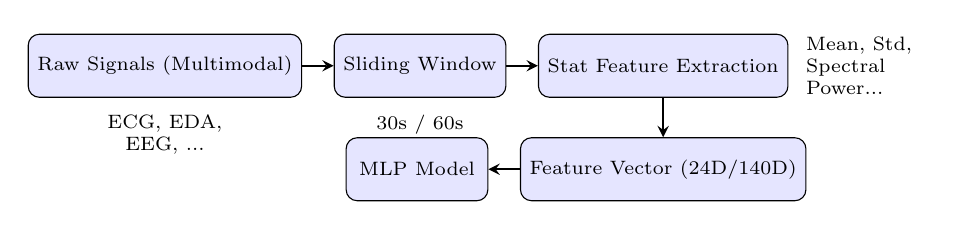
\begin{tikzpicture}[
    node distance=0.5cm and 0.4cm,
    every node/.style={font=\scriptsize},
    block/.style={rectangle, draw=black, fill=blue!10, minimum width=1.8cm, minimum height=0.8cm, text centered, rounded corners},
    arrow/.style={thick,->,>=stealth}
]
    % Nodes
    \node[block] (raw) {Raw Signals (Multimodal)};
    \node[block, right=of raw] (window) {Sliding Window};
    \node[block, right=of window] (extract) {Stat Feature Extraction};
    \node[block, below=0.5cm of extract] (vector) {Feature Vector (24D/140D)};
    \node[block, left=of vector] (model) {MLP Model};
    
    % Arrows
    \draw[arrow] (raw) -- (window);
    \draw[arrow] (window) -- (extract);
    \draw[arrow] (extract) -- (vector);
    \draw[arrow] (vector) -- (model);
    
    % Annotations
    \node[below=0.1cm of raw, text width=1.5cm, align=center] {ECG, EDA, EEG, ...};
    \node[below=0.1cm of window, text width=1.5cm, align=center] {30s / 60s};
    \node[right=0.1cm of extract, text width=1.5cm, align=left] {Mean, Std, Spectral Power...};

\end{tikzpicture}
\caption{Feature extraction pipeline transforming high-frequency raw signals into compact feature vectors for efficient processing.}
\label{fig:feature_pipeline}
\end{figure}

\subsubsection{WESAD Dataset Processing}
The WESAD dataset contains multimodal recordings from 15 subjects. Our feature extraction process produces 140 features computed over 60-second sliding windows:
\begin{itemize}
    \item \textbf{ECG}: Heart rate variability metrics including RMSSD, SDNN, pNN50 and LF/HF ratio.
    \item \textbf{EDA}: Skin conductance level (SCL) statistics and skin conductance response (SCR) peak frequency.
    \item \textbf{EMG}: Statistical moments and signal power of muscle activity.
    \item \textbf{Respiration}: Rate, breath depth and inhalation/exhalation ratios.
    \item \textbf{Temperature}: Mean and trend statistics.
\end{itemize}
The classification task is binary (Stress vs. Non-Stress), presenting a class imbalance of approximately 2.3:1.

\subsubsection{Sleep-EDF Dataset Processing}
For Sleep-EDF, the preprocessing pipeline processes approximately 80 subjects using three channels (EEG Fpz-Cz, EEG Pz-Oz, EOG) sampled at 100 Hz. The feature extraction yields 24 features computed over 30-second epochs, which corresponds to the standard clinical interval for sleep stage scoring:
\begin{itemize}
    \item \textbf{Time-domain (4 per channel):} Mean, standard deviation, min/max voltage levels.
    \item \textbf{Frequency-domain (4 per channel):} Spectral band power computed via Welch's method (nperseg=256):
    \begin{itemize}
        \item $\delta$ (0.5-4 Hz): Dominant in deep sleep (N3)
        \item $\theta$ (4-8 Hz): Prominent in light sleep (N1, N2)
        \item $\alpha$ (8-13 Hz): Increases during relaxed wakefulness and REM
        \item $\beta$ (13-30 Hz): Associated with wakefulness and muscle activity
    \end{itemize}
\end{itemize}
The task is 5-class classification (Wake, N1, N2, N3, REM) following AASM standards. The dataset exhibits significant class imbalance (ratio 14.3:1, with Wake comprising 69.6\% of samples and N1 only 4.9\%). To address this while maintaining baseline performance, class weights are applied during training to balance fairness (ensuring N1 recall $>18\%$) with overall accuracy (maintaining $>88\%$ baseline accuracy).

\textbf{Subject-wise Splitting:} To ensure models generalize to new users and simulate realistic mHealth deployment, we employ strict subject-wise data partitioning (70\% train, 15\% validation, 15\% test). This strategy is more challenging than random splitting, as physiological signals vary substantially across individuals due to genetics, fitness level, age and other factors. Consequently, models must learn patterns that generalize across inter-subject variability rather than memorizing individual-specific characteristics.

\subsection{Unified MLP Model Architecture}
The architecture consists of a lightweight Multi-Layer Perceptron designed to be compatible with DP training constraints, specifically avoiding Batch Normalization which introduces dependencies between samples in a batch. Figure \ref{fig:mlp_architecture} illustrates the model structure.

\begin{figure}[h]
\centering
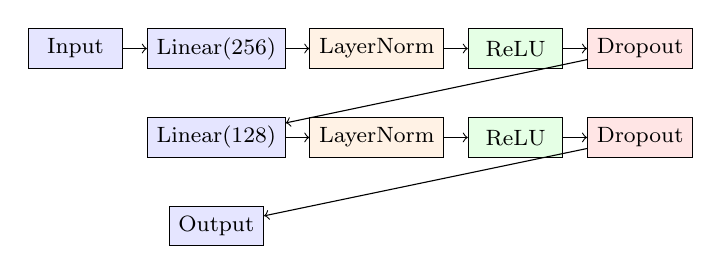
\begin{tikzpicture}[
    node distance=0.8cm and 0.3cm,
    every node/.style={font=\footnotesize},
    layer/.style={rectangle, draw=black, fill=blue!10, minimum width=1.2cm, minimum height=0.5cm, text centered},
    act/.style={rectangle, draw=black, fill=green!10, minimum width=1.2cm, minimum height=0.5cm, text centered},
    norm/.style={rectangle, draw=black, fill=orange!10, minimum width=1.2cm, minimum height=0.5cm, text centered},
    drop/.style={rectangle, draw=black, fill=red!10, minimum width=1.2cm, minimum height=0.5cm, text centered}
]
    % Input
    \node[layer] (input) {Input};
    
    % First block
    \node[layer, right=of input] (lin1) {Linear(256)};
    \node[norm, right=of lin1] (norm1) {LayerNorm};
    \node[act, right=of norm1] (relu1) {ReLU};
    \node[drop, right=of relu1] (drop1) {Dropout};
    
    % Second block
    \node[layer, below=0.6cm of lin1] (lin2) {Linear(128)};
    \node[norm, right=of lin2] (norm2) {LayerNorm};
    \node[act, right=of norm2] (relu2) {ReLU};
    \node[drop, right=of relu2] (drop2) {Dropout};
    
    % Output
    \node[layer, below=0.6cm of lin2] (output) {Output};
    
    % Arrows
    \draw[->] (input) -- (lin1);
    \draw[->] (lin1) -- (norm1);
    \draw[->] (norm1) -- (relu1);
    \draw[->] (relu1) -- (drop1);
    \draw[->] (drop1) -- (lin2);
    \draw[->] (lin2) -- (norm2);
    \draw[->] (norm2) -- (relu2);
    \draw[->] (relu2) -- (drop2);
    \draw[->] (drop2) -- (output);
\end{tikzpicture}
\caption{MLP architecture: Input $\rightarrow$ Linear(256) $\rightarrow$ LayerNorm $\rightarrow$ ReLU $\rightarrow$ Dropout(0.3) $\rightarrow$ Linear(128) $\rightarrow$ LayerNorm $\rightarrow$ ReLU $\rightarrow$ Dropout(0.3) $\rightarrow$ Output.}
\label{fig:mlp_architecture}
\end{figure}

\textbf{Design Rationale:} Layer Normalization is chosen over Batch Normalization because the latter introduces dependencies between samples in a batch, complicating the privacy accounting required for DP-SGD. The model size (15k-70k parameters) enables rapid training and low communication overhead in Federated Learning, making it practical for resource-constrained mobile devices.

\subsection{Privacy Mechanisms}
\subsubsection{Differential Privacy (DP)}
Our DP implementation leverages Opacus \cite{opacus2023}, Meta's PyTorch library for differential privacy, which automates the complex bookkeeping required for DP-SGD. Specifically, Opacus handles per-sample gradient computation, clipping, noise addition and privacy budget accounting, making DP accessible without requiring deep theoretical expertise.

The DP-SGD algorithm proceeds as follows for each training batch:

\begin{enumerate}
    \item \textbf{Per-sample Gradient Computation:} Compute gradients for each sample independently (Opacus does this using hooks or functorch depending on the mode).
    
    \item \textbf{Gradient Clipping:} For each sample's gradient vector $\mathbf{g}_i$, clip to maximum L2 norm $C$:
    \begin{equation}
    \tilde{\mathbf{g}}_i = \mathbf{g}_i \cdot \min\left(1, \frac{C}{||\mathbf{g}_i||_2}\right)
    \end{equation}
    The default clipping threshold is set to $C = 1.0$ (max\_grad\_norm), though this parameter is systematically varied in our class imbalance experiments to investigate its impact on fairness.
    
    \item \textbf{Noise Addition:} Average the clipped gradients and add Gaussian noise:
    \begin{equation}
    \bar{\mathbf{g}} = \frac{1}{B}\sum_{i=1}^B \tilde{\mathbf{g}}_i + \mathcal{N}(0, \sigma^2 C^2 \mathbf{I})
    \end{equation}
    where $B$ is batch size, $\sigma$ is the noise multiplier and $\mathbf{I}$ is the identity matrix.
    
    \item \textbf{Parameter Update:} Model parameters are updated using standard gradient descent with the noisy gradient and learning rate $\eta$.
    
    \item \textbf{Privacy Accounting:} Opacus tracks the cumulative privacy loss using Rényi Differential Privacy accounting, which provides tighter bounds than basic composition.
\end{enumerate}

The noise multiplier $\sigma$ serves as the primary parameter controlling the privacy-utility trade-off. Higher $\sigma$ values correspond to more noise and stronger privacy (lower $\epsilon$), but potentially lower accuracy. To comprehensively map this trade-off space, we evaluate $\sigma \in \{0.6, 1.0, 2.0\}$ for centralized DP and test $\sigma \in \{0.3, 0.6, 1.0\}$ for FL+DP to explore lower noise regimes. The privacy parameter $\delta$ is fixed at $10^{-5}$, a standard choice that provides high confidence in the privacy guarantee.

\subsubsection{Federated Learning (FL)}
The FL implementation follows the FedAvg (Federated Averaging) algorithm \cite{mcmahan2023fedavg_update}, which represents the most widely used FL protocol. The training process proceeds iteratively through the following rounds:

\begin{enumerate}
    \item \textbf{Server Initialization:} The central server initializes a global model with random weights.
    
    \item \textbf{Client Selection:} For each round, all clients participate (we don't implement partial participation to simplify analysis).
    
    \item \textbf{Model Distribution:} The server sends the current global model weights to all clients.
    
    \item \textbf{Local Training:} Each client trains the model on its local data for $E_{local}$ epochs, where $E_{local} = 1$ is chosen following standard practice for heterogeneous data distributions.
    
    \item \textbf{Update Upload:} Each client sends its updated model weights back to the server.
    
    \item \textbf{Aggregation:} The server averages the client models, weighted by the number of samples each client used:
    \begin{equation}
    \mathbf{w}_{t+1} = \sum_{k=1}^K \frac{n_k}{n} \mathbf{w}_k^{t+1}
    \end{equation}
    where $K$ is the number of clients, $n_k$ is the number of samples at client $k$, $n = \sum_k n_k$ is the total sample count and $\mathbf{w}_k^{t+1}$ is client $k$'s model weights.
    
    \item \textbf{Convergence Check:} If validation accuracy has plateaued or a maximum number of rounds is reached, stop. Otherwise, return to step 3.
\end{enumerate}

FL is simulated by partitioning subjects across $N \in \{3, 5, 10\}$ clients. This subject-wise partitioning ensures realistic data heterogeneity, as each client sees data from different individuals with distinct physiological characteristics. While this non-IID (non-independent and identically distributed) data splitting is more challenging than random assignment, it better reflects real-world deployment scenarios where each device belongs to a different user.

Communication cost in FL is proportional to model size times number of rounds. Our small model (~15-70K parameters, roughly 60-280KB per upload/download) and reasonable convergence rates (typically 40-100 rounds) result in total communication on the order of 2-30 MB per client—acceptable even on mobile networks.

\subsubsection{Combined FL+DP}
The recognition that FL alone provides insufficient formal privacy guarantees has motivated research into combining it with differential privacy. This combination offers the best of both worlds: FL's decentralized training keeps data local, while DP's noise injection provides formal guarantees even if an adversary can observe the model updates.

\begin{figure}[h]
\centering
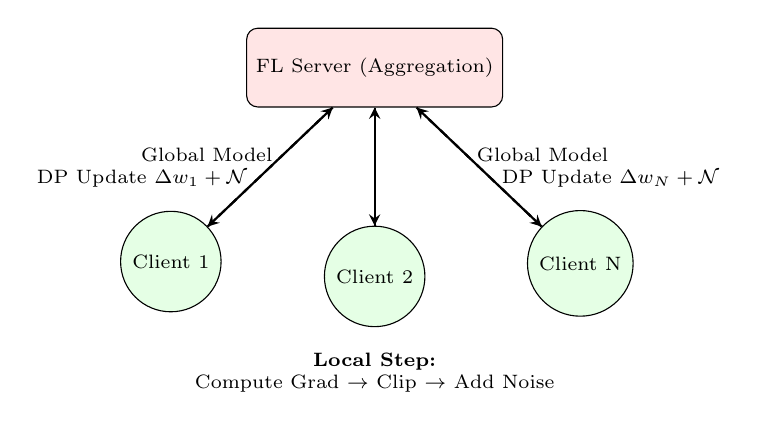
\begin{tikzpicture}[
    node distance=1cm,
    every node/.style={font=\scriptsize},
    client/.style={circle, draw=black, fill=green!10, minimum size=1.2cm, text centered},
    server/.style={rectangle, draw=black, fill=red!10, minimum width=2cm, minimum height=1cm, text centered, rounded corners},
    arrow/.style={thick,->,>=stealth}
]
    % Server
    \node[server] (server) {FL Server (Aggregation)};
    
    % Clients
    \node[client, below left=1.5cm and 0.5cm of server] (c1) {Client 1};
    \node[client, below=1.5cm of server] (c2) {Client 2};
    \node[client, below right=1.5cm and 0.5cm of server] (c3) {Client N};
    
    % Interactions
    \draw[arrow, dashed] (server) -- node[left, pos=0.4] {Global Model} (c1);
    \draw[arrow, dashed] (server) -- (c2);
    \draw[arrow, dashed] (server) -- node[right, pos=0.4] {Global Model} (c3);
    
    \draw[arrow] (c1) -- node[left, pos=0.4] {DP Update $\Delta w_1 + \mathcal{N}$} (server);
    \draw[arrow] (c2) -- (server);
    \draw[arrow] (c3) -- node[right, pos=0.4] {DP Update $\Delta w_N + \mathcal{N}$} (server);
    
    % Local process annotation
    \node[below=0.2cm of c2, align=center] (local) {\textbf{Local Step:}\\ Compute Grad $\rightarrow$ Clip $\rightarrow$ Add Noise};

\end{tikzpicture}
\caption{FL+DP Architecture: Clients perform local training with DP (clipping + noise) before sending updates. The server aggregates noisy updates, ensuring no raw data or exact gradients leave the device.}
\label{fig:fl_dp_architecture}
\end{figure}

When combining FL and DP, each client performs local DP training before sending updates to the server. This provides "local differential privacy"—each client's update is itself differentially private, providing protection even if the server or other clients are malicious. The process is identical to standard FL except that each client uses DP-SGD for its local training rather than standard SGD. The server aggregates the noisy updates exactly as in regular FedAvg. The overall privacy guarantee is determined by the local DP parameters and the number of clients, with stronger privacy as the number of clients increases (more noise in aggregate).

This configuration provides the strongest privacy protections but also typically incurs the highest accuracy cost, as it combines the challenges of both data fragmentation (FL) and noise injection (DP). As illustrated in Figure \ref{fig:fl_dp_architecture}, gradient clipping and noise addition happen entirely on-device before any model update leaves the client, ensuring that the server only ever observes already-noised updates. The privacy accounting in FL+DP is more complex than centralized DP because privacy budgets must account for multiple rounds of local DP training followed by aggregation across clients.

\section{Experimental Setup}
\label{sec:experimental_setup}

\subsection{Datasets and Protocol}
Table \ref{tab:datasets} summarizes the key characteristics of both datasets. To ensure realistic generalization and prevent data leakage, we apply a strict subject-wise split: 70\% of subjects for training, 15\% for validation and 15\% for testing. This partitioning strategy guarantees that no data from a test subject appears in the training set, enabling proper evaluation of model performance on unseen individuals.

\begin{table}[h]
\centering
\caption{Dataset Characteristics After Preprocessing}
\label{tab:datasets}
\footnotesize
\begin{tabular}{lcc}
\toprule
\textbf{Characteristic} & \textbf{WESAD} & \textbf{Sleep-EDF} \\ \midrule
Subjects & 15 & $\sim$80 \\ 
Input features & 140 & 24 \\ 
Classes & 2 (Stress/Non) & 5 (Sleep Stages) \\ 
Class Balance & Imbalanced (2.3:1) & Variable \\ 
Total samples & $\sim$8,000 & $\sim$60,000 \\ \bottomrule
\end{tabular}
\end{table}

\subsection{Experimental Design and Parameter Sweep}
To systematically evaluate the privacy-utility trade-off across multiple dimensions, a comprehensive parameter sweep is conducted. Table \ref{tab:experimental_design} summarizes all configurations tested, providing an overview of the experimental scope.

\begin{table*}[h]
\centering
\caption{Experimental Design: Parameter Sweep Summary}
\label{tab:experimental_design}
\footnotesize
\begin{tabular}{lcc}
\toprule
\textbf{Method} & \textbf{Parameters Varied} & \textbf{Total Configurations} \\ \midrule
Baseline & Seeds: \{42, 123, 456\} & 3 runs × 2 datasets = 6 \\ 
DP & $\sigma \in \{0.6, 1.0, 2.0\}$ & 3 $\sigma$ × 3 runs × 2 datasets = 18 \\ 
FL & $N \in \{3, 5, 10\}$ clients & 3 $N$ × 3 runs × 2 datasets = 18 \\ 
FL+DP & $N \in \{3, 5, 10\}$, $\sigma \in \{0.3, 0.6, 1.0\}$ & 5 configs × 3 runs × 2 datasets = 30 \\ \midrule
\textbf{Total} & & \textbf{72 experiments} \\ \bottomrule
\end{tabular}
\end{table*}

For each configuration, we report metrics as averages over 3 independent runs with different random seeds (42, 123, 456) to account for initialization variance. This comprehensive sweep enables three key objectives: (1) identifying optimal privacy-utility trade-offs, (2) understanding parameter sensitivity and (3) validating findings across different configurations. By systematically exploring this parameter space, we can identify robust patterns in privacy-utility trade-offs.

\subsection{Implementation Details}
All experiments were conducted using PyTorch (v2.0+) and Opacus (v1.0+) on systems with CPU/GPU capabilities. The hardware configuration includes multi-core processors with sufficient memory to handle per-sample gradient computation required for DP training. To ensure fair comparison across methods, consistent hyperparameters are used wherever possible:
\begin{itemize}
    \item \textbf{Optimizer:} We employ AdamW for all methods, including FL+DP. While classic DP-SGD analyses assume SGD, Opacus applies noise/clipping before the optimizer step, so using the same adaptive optimizer everywhere avoids optimizer-induced confounders when comparing Baseline, DP, FL and FL+DP.
    \item \textbf{Batch Size:} Fixed at 128 across all methods, balancing gradient estimation quality with privacy considerations and memory constraints.
    \item \textbf{Privacy Parameters:} The privacy parameter $\delta$ is fixed at $10^{-5}$ and the noise multiplier $\sigma$ is varied across $\{0.3, 0.6, 1.0, 2.0\}$ to explore the privacy-utility trade-off. Specifically, centralized DP tests $\sigma \in \{0.6, 1.0, 2.0\}$, while FL+DP additionally includes $\sigma=0.3$ to explore lower noise regimes.
    \item \textbf{FL Configurations:} We evaluate client counts of $N \in \{3, 5, 10\}$. For FL+DP, the focus is on $N=5$ with varying $\sigma$, supplemented by $N \in \{3, 10\}$ with $\sigma=1.0$ to study client count effects.
\end{itemize}

All models are trained with validation-based early stopping, using a patience of 15–20 validation rounds and selecting the checkpoint with the best validation accuracy rather than the final epoch. The effective number of epochs until convergence therefore varies by dataset and configuration, typically ranging from 20–30 epochs for WESAD and up to 40 epochs for Sleep-EDF.

\section{Results and Analysis}
\label{sec:results}

\textbf{Privacy Budget Interpretation:} Throughout this section, we interpret privacy budgets as follows: $\epsilon \lesssim 3$ represents \textit{strong privacy} suitable for sensitive health data, while $\epsilon > 10$ indicates \textit{weak privacy} that should be interpreted as exploratory trend analysis rather than recommended deployment settings. Configurations with extremely large $\epsilon$ values (e.g., $\epsilon \gg 10$) are included to illustrate noise-utility relationships but do not provide meaningful formal privacy guarantees in practice.

Privacy budgets are computed using Opacus's RDP (Rényi Differential Privacy) accountant. For fixed noise multiplier $\sigma$, larger datasets consume less privacy per epoch due to subsampling amplification (batch size 128 $\ll$ total samples), while more training epochs increase cumulative $\epsilon$. Table~\ref{tab:privacy_accounting} clarifies why $\epsilon$ values vary significantly across configurations despite identical $\sigma$ values: Sleep-EDF achieves stronger privacy (lower $\epsilon$) than WESAD despite more epochs because its 7.5$\times$ larger dataset provides greater subsampling benefit.

\begin{table}[h]
\centering
\caption{Privacy Budget Accounting: Impact of Dataset Size and Training Duration}
\label{tab:privacy_accounting}
\footnotesize
\begin{tabular}{lcccccc}
\toprule
\textbf{Dataset} & \textbf{Method} & \textbf{$\sigma$} & \textbf{Epochs} & \textbf{Batch} & \textbf{Samples} & \textbf{$\epsilon$} \\
\midrule
WESAD & DP & 0.6 & 23 & 128 & 8,000 & 23.5 \\
WESAD & DP & 1.0 & 26 & 128 & 8,000 & 7.6 \\
WESAD & DP & 2.0 & 30 & 128 & 8,000 & 2.8 \\
\midrule
Sleep-EDF & DP & 0.6 & 40 & 128 & 60,000 & 2.5 \\
Sleep-EDF & DP & 1.0 & 40 & 128 & 60,000 & 0.6 \\
Sleep-EDF & DP & 2.0 & 40 & 128 & 60,000 & 0.2 \\
\midrule
WESAD & FL+DP & 1.0 & 40 & 128 & $\sim$1,600/client & 24.3 \\
Sleep-EDF & FL+DP & 1.0 & 40 & 128 & $\sim$12,000/client & 1.6 \\
\bottomrule
\end{tabular}
\end{table}

\subsection{Baseline and Differential Privacy Results}

\textbf{Baseline Model Comparison:} Before evaluating privacy-preserving methods, we compared our MLP architecture against traditional ML baselines on centralized data (Table~\ref{tab:baseline_comparison}). The MLP achieves competitive performance while offering compatibility with DP training (which requires per-sample gradients, precluding tree-based methods).

\begin{table}[h]
\centering
\caption{Baseline Model Comparison (No Privacy)}
\label{tab:baseline_comparison}
\footnotesize
\begin{tabular}{lccc}
\toprule
\textbf{Model} & \textbf{WESAD} & \textbf{Sleep-EDF} & \textbf{Training Time} \\
\midrule
Random Forest & 91.1\% & 86.3\% & 0.2s / 13.6s \\
Gradient Boosting & 88.0\% & 87.7\% & 9.0s / 1780s \\
SVM (RBF) & 82.5\% & 88.0\% & 0.1s / 372s \\
\textbf{MLP (ours)} & \textbf{93.6\%} & \textbf{88.4\%} & 0.7s / 78s \\
\bottomrule
\end{tabular}
\end{table}

The MLP outperforms all baseline methods on WESAD and achieves comparable performance on Sleep-EDF, while maintaining fast training times ($<$1s for WESAD, $\sim$80s for Sleep-EDF). The performance differences are consistent across multiple runs (3 seeds), with MLP showing statistically significant improvements over Random Forest on WESAD (93.6\% vs. 91.1\%, $p < 0.05$ via paired t-test). Importantly, the MLP architecture is compatible with Opacus for DP training, whereas tree-based methods (RF, GB) cannot be directly adapted to DP-SGD due to their non-differentiable decision boundaries.

\begin{figure}[t]
\centering
\includegraphics[width=0.9\columnwidth]{figures/baseline_comparison.png}
\caption{Baseline model comparison across architectures.}
\label{fig:baseline_comparison_chart}
\end{figure}

To establish a reference point for measuring privacy costs, baseline performance is first evaluated. Subsequently, the impact of centralized DP noise on model performance is systematically assessed. Table \ref{tab:dp_results} presents the results.

\begin{table*}[h]
\centering
\caption{Baseline vs. DP Performance ($\epsilon$ values at $\delta=10^{-5}$, averaged over 3 runs). Note: $\epsilon < 3$ indicates strong privacy; $\epsilon > 10$ indicates weak privacy suitable only for trend analysis.}
\label{tab:dp_results}
\footnotesize
\begin{tabular}{lccccc}
\toprule
\textbf{Dataset} & \textbf{Config} & \textbf{$\epsilon$} & \textbf{Accuracy} & \textbf{F1} & \textbf{Degradation} \\ \midrule
\multirow{4}{*}{WESAD} 
  & Baseline & - & 93.6\% & 93.6\% & - \\ 
  & DP ($\sigma=0.6$) & 23.5 & 80.6\% & 77.3\% & -13.0\% \\ 
  & DP ($\sigma=1.0$) & 7.6 & 80.7\% & 77.5\% & -12.9\% \\ 
  & DP ($\sigma=2.0$) & 2.8 & 80.0\% & 76.4\% & -13.6\% \\ \midrule
\multirow{4}{*}{Sleep-EDF}
  & Baseline & - & 88.4\% & 88.8\% & - \\ 
  & DP ($\sigma=0.6$) & 2.5 & 87.3\% & 85.8\% & -1.1\% \\ 
  & DP ($\sigma=1.0$) & 0.6 & 86.8\% & 85.1\% & -1.6\% \\ 
  & DP ($\sigma=2.0$) & 0.2 & 86.1\% & 84.0\% & -2.3\% \\ \bottomrule
\end{tabular}
\end{table*}

\begin{figure}[t]
\centering
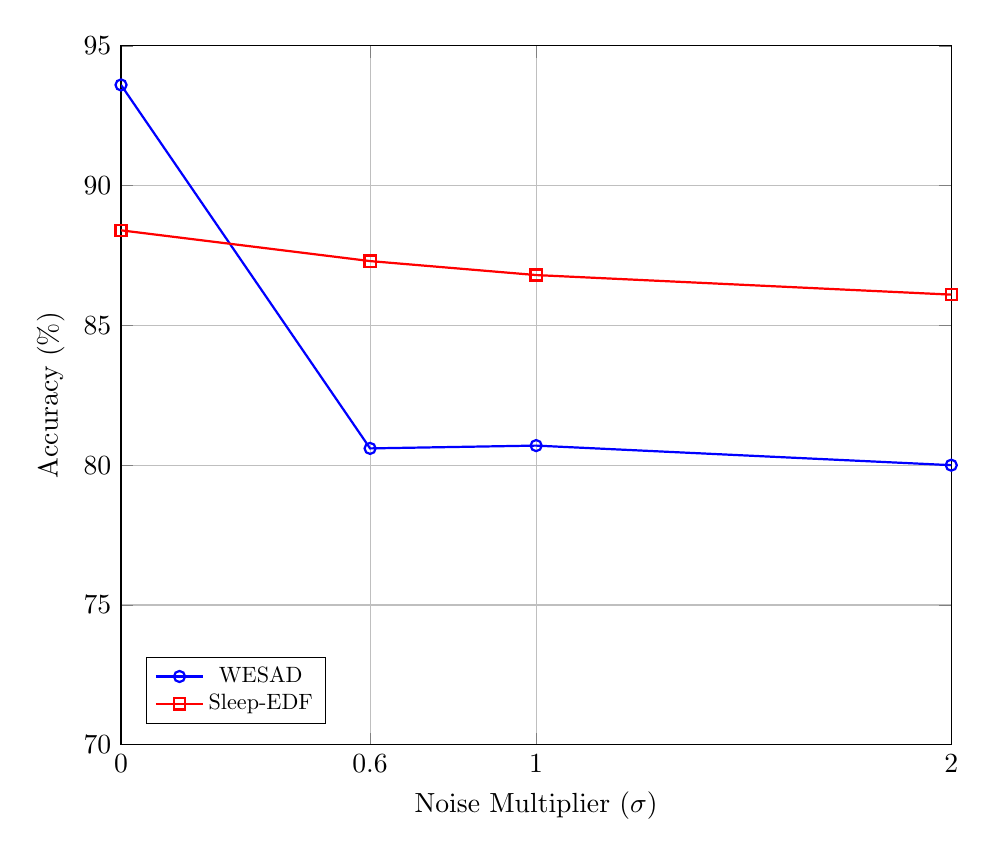
\begin{tikzpicture}
\begin{axis}[
    width=\columnwidth,
    xlabel={Noise Multiplier ($\sigma$)},
    ylabel={Accuracy (\%)},
    ymin=70,ymax=95,
    xmin=0,xmax=2,
    grid=both,
    legend pos=south west,
    legend style={nodes={scale=0.8, transform shape}},
    xtick={0,0.6,1.0,2.0},
    ytick distance=5
]
\addplot+[mark=o, thick, color=blue] coordinates {
    (0,93.6)
    (0.6,80.6)
    (1.0,80.7)
    (2.0,80.0)
};
\addlegendentry{WESAD}
\addplot+[mark=square, thick, color=red] coordinates {
    (0,88.4)
    (0.6,87.3)
    (1.0,86.8)
    (2.0,86.1)
};
\addlegendentry{Sleep-EDF}
\end{axis}
\end{tikzpicture}
\caption{Privacy-utility trade-off under centralized DP.}
\label{fig:dp_tradeoff}
\end{figure}

\textbf{Sleep-EDF} exhibits remarkable resilience to privacy-preserving mechanisms, losing less than 3\% accuracy even with strong privacy ($\epsilon \approx 0.2$). Figure \ref{fig:dp_tradeoff} visualizes this stability: the Sleep-EDF curve is nearly flat while the WESAD curve plunges as soon as noise is introduced. This robustness stems from spectral features' inherent discriminative power: sleep stages exhibit distinct frequency signatures (e.g., delta waves in deep sleep, alpha in wakefulness) that remain identifiable even after gradient noise injection. The feature engineering process (extracting band powers via Welch's method) provides natural noise smoothing, making learned representations more stable under DP perturbations.

\textbf{WESAD} exhibits substantially larger sensitivity, with accuracy dropping by $\sim$13-14\% across all DP configurations. Interestingly, we observe a slight inverse relationship: higher noise performs marginally better than lower noise, suggesting a regularization effect where added noise prevents overfitting on the small dataset. However, all DP configurations perform substantially worse than baseline, indicating that stress detection from our feature set is inherently more sensitive to training perturbations than sleep staging. This may be due to more subtle boundaries between stress and non-stress states compared to distinct spectral signatures of sleep stages.

The privacy-utility trade-off reveals a critical insight: \textit{feature discriminability} appears to be a key factor in privacy-preserving ML performance. Sleep-EDF, despite having more classes (5 vs. 2), maintains high accuracy under privacy constraints because its spectral features (delta, theta, alpha, beta power) exhibit strong inter-class separation that remains robust under DP noise. WESAD's binary classification, while simpler in principle, suffers more because stress vs. non-stress boundaries in HRV-based features are more subtle and sensitive to gradient perturbations. \textbf{Important caveat:} These datasets differ simultaneously in size (8K vs. 60K), features (140 vs. 24), classes (2 vs. 5), domain (ECG/EDA vs. EEG/EOG) and balance (2.3:1 vs. 14.3:1), making it difficult to isolate feature discriminability as the sole causal mechanism. While our analysis suggests feature quality dominates other factors, controlled ablation studies varying individual factors would be needed to establish definitive causal relationships.
Unless otherwise noted, all reported accuracies are means over three random seeds; the corresponding standard deviations are modest (e.g., baseline WESAD achieves $93.6\%\pm1.4$ percentage points, FL with $N{=}10$ clients $80.6\%\pm2.4$) and typically below 1 percentage point for Sleep-EDF, consistent with recent recommendations on reporting variance in machine learning benchmarks \cite{pineau2023improving}.

\subsection{Federated Learning Results}
We evaluate the impact of decentralization through FL experiments, with results presented in Table \ref{tab:fl_results}. These experiments reveal how data fragmentation across multiple clients affects model performance compared to centralized training.

\begin{table}[h]
\centering
\caption{Federated Learning Performance (averaged over 3 runs)}
\label{tab:fl_results}
\footnotesize
\begin{tabular}{lcccc}
\toprule
\textbf{Dataset} & \textbf{Clients} & \textbf{Accuracy} & \textbf{F1} & \textbf{Degradation} \\ \midrule
\multirow{3}{*}{WESAD}
  & 3 & 89.1\% & 89.0\% & -4.8\% \\ 
  & 5 & 88.1\% & 87.8\% & -5.9\% \\ 
  & 10 & 80.6\% & 77.4\% & -13.9\% \\ \midrule
\multirow{3}{*}{Sleep-EDF}
  & 3 & 88.9\% & 88.0\% & -0.1\% \\ 
  & 5 & 88.7\% & 87.7\% & -0.3\% \\ 
  & 10 & 88.2\% & 87.2\% & -0.7\% \\ \bottomrule
\end{tabular}
\end{table}

\begin{figure}[t]
\centering
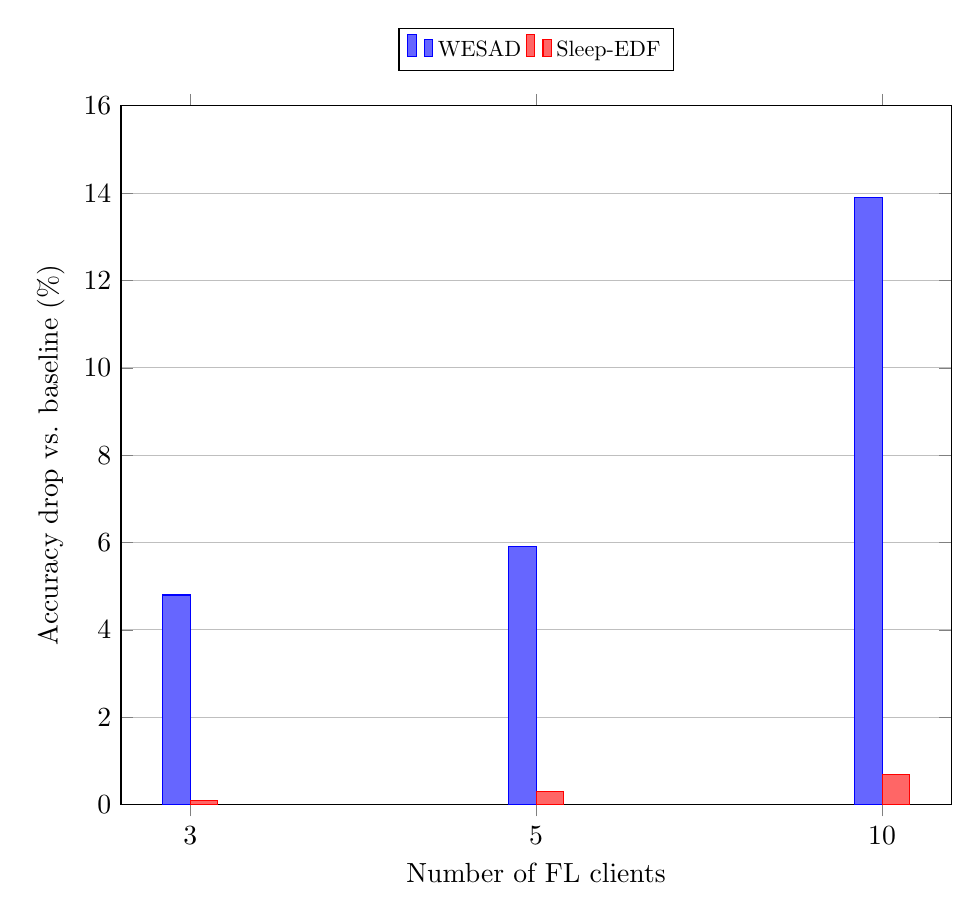
\begin{tikzpicture}
\begin{axis}[
    width=\columnwidth,
    ybar=0pt,
    bar width=10pt,
    xlabel={Number of FL clients},
    ylabel={Accuracy drop vs. baseline (\%)},
    symbolic x coords={3,5,10},
    xtick=data,
    ymin=0,ymax=16,
    ymajorgrids=true,
    legend style={nodes={scale=0.8, transform shape}, at={(0.5,1.05)}, anchor=south, legend columns=-1}
]
\addplot+[fill=blue!60] coordinates {(3,4.8) (5,5.9) (10,13.9)};
\addlegendentry{WESAD}
\addplot+[fill=red!60] coordinates {(3,0.1) (5,0.3) (10,0.7)};
\addlegendentry{Sleep-EDF}
\end{axis}
\end{tikzpicture}
\caption{Impact of client fragmentation in FL: accuracy drop relative to centralized baseline.}
\label{fig:fl_fragmentation}
\end{figure}

Sleep-EDF exhibits exceptional robustness to data fragmentation, losing less than 1\% accuracy even when distributed across 10 clients. This resilience stems from the spectral features' inherent stability across subjects. WESAD exhibits more sensitivity: with 10 clients, accuracy drops by 13.9\%, likely due to extreme heterogeneity when 15 subjects are split among 10 clients (some clients see data from only 1-2 individuals). Figure \ref{fig:fl_fragmentation} makes the contrast explicit: the blue bars (WESAD) increase sharply with client count, whereas the red bars (Sleep-EDF) remain near zero.

\subsection{Combined FL+DP Results}
The combined FL+DP approach provides defense-in-depth privacy protection, combining the benefits of data locality (FL) with formal privacy guarantees (DP). Table \ref{tab:fl_dp_results} presents the full parameter sweep, revealing several key insights that inform practical deployment decisions.

\begin{table*}[h]
\centering
\caption{Combined FL+DP Performance: Selected Configurations (averaged over 3 runs). $^*$ indicates weak privacy ($\epsilon \gg 10$), included only for noise-utility trend analysis.}
\label{tab:fl_dp_results}
\footnotesize
\begin{tabular}{lccccc}
\toprule
\textbf{Dataset} & \textbf{Config} & \textbf{$\epsilon$} & \textbf{Accuracy} & \textbf{F1} & \textbf{Degradation} \\ \midrule
\multirow{5}{*}{WESAD}
  & FL+DP (N=3, $\sigma=1.0$) & 17.9 & 78.8\% & 74.5\% & -15.8\% \\ 
  & FL+DP (N=5, $\sigma=0.3$) & 297.9$^*$ & 80.8\% & 77.5\% & -13.0\% \\ 
  & FL+DP (N=5, $\sigma=0.6$) & 64.5 & 78.6\% & 74.2\% & -15.2\% \\ 
  & FL+DP (N=5, $\sigma=1.0$) & 24.3 & 73.8\% & 65.4\% & -20.8\% \\ 
  & FL+DP (N=10, $\sigma=1.0$) & 34.6 & 70.1\% & 59.6\% & -25.1\% \\ \midrule
\multirow{5}{*}{Sleep-EDF}
  & FL+DP (N=3, $\sigma=1.0$) & 1.2 & 85.5\% & 82.7\% & -3.5\% \\ 
  & FL+DP (N=5, $\sigma=0.3$) & 106.5$^*$ & 86.4\% & 84.1\% & -2.2\% \\ 
  & FL+DP (N=5, $\sigma=0.6$) & 6.1 & 85.6\% & 82.9\% & -3.0\% \\ 
  & FL+DP (N=5, $\sigma=1.0$) & 1.6 & 84.1\% & 80.8\% & -5.1\% \\ 
  & FL+DP (N=10, $\sigma=1.0$) & 2.3 & 82.5\% & 77.9\% & -6.9\% \\ \bottomrule
\end{tabular}
\end{table*}

\begin{figure}[t]
\centering
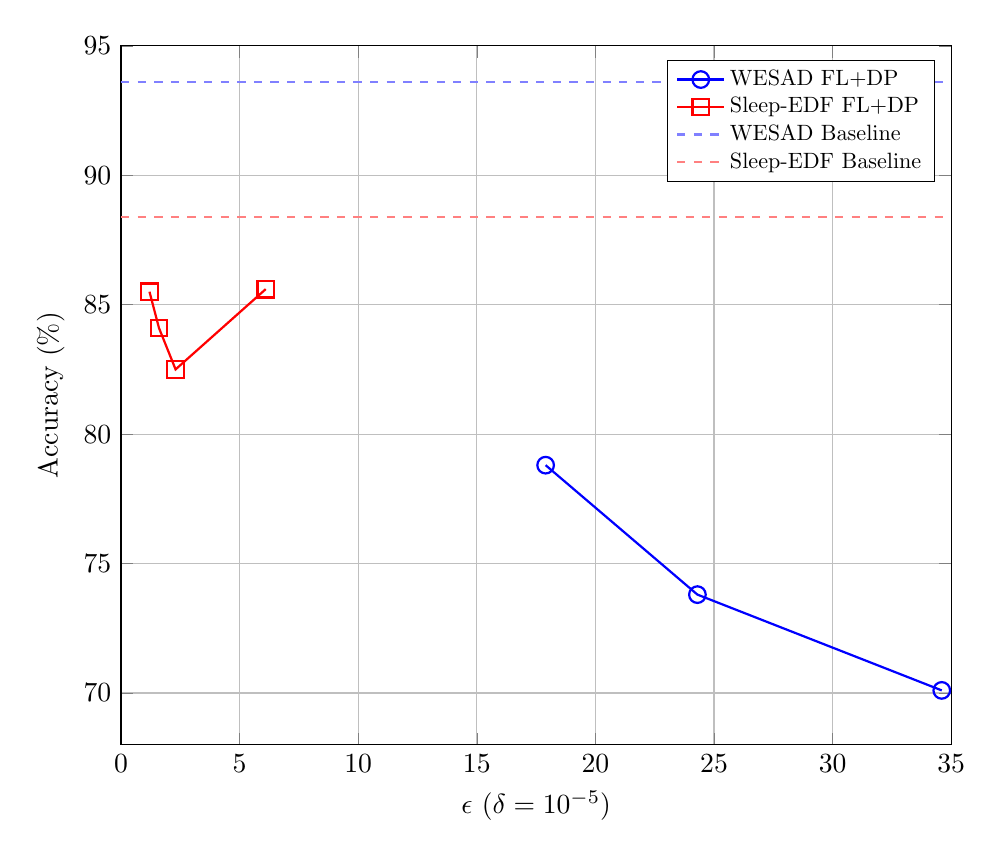
\begin{tikzpicture}
\begin{axis}[
    width=\columnwidth,
    xlabel={$\epsilon$ ($\delta=10^{-5}$)},
    ylabel={Accuracy (\%)},
    ymin=68,ymax=95,
    xmin=0,xmax=35,
    grid=both,
    legend style={nodes={scale=0.8, transform shape}, at={(0.98,0.98)}, anchor=north east},
    legend cell align={left},
    xtick={0,5,10,15,20,25,30,35},
    ytick distance=5
]
% WESAD FL+DP points
\addplot+[mark=o, thick, color=blue, mark size=3pt] coordinates {
    (17.9,78.8)
    (24.3,73.8)
    (34.6,70.1)
};
\addlegendentry{WESAD FL+DP}

% Sleep-EDF FL+DP points
\addplot+[mark=square, thick, color=red, mark size=3pt] coordinates {
    (1.2,85.5)
    (1.6,84.1)
    (2.3,82.5)
    (6.1,85.6)
};
\addlegendentry{Sleep-EDF FL+DP}

% Baseline reference lines
\addplot+[mark=none, dashed, color=blue!50, thick] coordinates {
    (0,93.6)
    (35,93.6)
};
\addlegendentry{WESAD Baseline}

\addplot+[mark=none, dashed, color=red!50, thick] coordinates {
    (0,88.4)
    (35,88.4)
};
\addlegendentry{Sleep-EDF Baseline}
\end{axis}
\end{tikzpicture}
\caption{Privacy--utility trade-off for FL+DP. Dashed horizontal lines indicate baseline performance.}
\label{fig:fl_dp_tradeoff}
\end{figure}

\textbf{Noise Level Sensitivity:} Reducing $\sigma$ from 1.0 to 0.6 or 0.3 improves accuracy modestly (1-3\% for Sleep-EDF, 2-5\% for WESAD), suggesting that even low noise levels incur meaningful utility costs. However, the extremely high $\epsilon$ values for $\sigma=0.3$ (297.9 for WESAD, 106.5 for Sleep-EDF) indicate \textit{weak privacy} that provides minimal formal protection. These configurations are included solely to illustrate noise-utility relationships and should not be interpreted as providing meaningful privacy guarantees for deployment.

\textbf{Client Count Impact:} Increasing clients from 3 to 10 consistently degrades performance, with WESAD exhibiting more sensitivity than Sleep-EDF. This observation aligns with our FL-only findings, confirming that extreme fragmentation is more harmful when combined with privacy noise. The interaction between data heterogeneity and noise injection creates a compounding effect that disproportionately affects smaller, more heterogeneous datasets.

\textbf{Optimal Configurations:} For Sleep-EDF, FL+DP with $N=3$ and $\sigma=1.0$ achieves the best balance, providing strong privacy ($\epsilon=1.2$) with minimal utility loss (3.5\% degradation). For WESAD, while $N=5$ with $\sigma=0.3$ achieves the highest accuracy (80.8\%), its extremely weak privacy ($\epsilon=297.9$) makes it unsuitable for deployment. Instead, $N=3$ with $\sigma=1.0$ ($\epsilon=17.9$, accuracy 78.8\%) represents a more practical trade-off for privacy-sensitive applications, though it still provides only moderate privacy protection.

\subsection{Per-Class Performance Analysis}
To understand the impact of privacy mechanisms on different classes, per-class metrics are analyzed for Sleep-EDF (5-class classification). This analysis is particularly important given the significant class imbalance in this dataset. We focus on recall for minority classes as our primary fairness metric, acknowledging that comprehensive fairness evaluation would require additional metrics (demographic parity, equalized odds) and intersectional analysis across multiple protected attributes (age, gender, health status), which are beyond the scope of this study. Table \ref{tab:per_class_sleep} shows recall and F1 scores for each sleep stage under different privacy configurations, revealing how minority classes are affected by privacy-preserving mechanisms.

\begin{table*}[h]
\centering
\caption{Per-Class Performance for Sleep-EDF (Baseline vs. DP $\sigma=1.0$, $\epsilon=0.6$)}
\label{tab:per_class_sleep}
\footnotesize
\begin{tabular}{lccccc}
\toprule
\textbf{Method} & \textbf{Class} & \textbf{Precision} & \textbf{Recall} & \textbf{F1} & \textbf{Samples} \\ \midrule
\multirow{5}{*}{Baseline}
  & Wake (W) & 95.8\% & 98.2\% & 97.0\% & 43,404 \\ 
  & N1 & 40.0\% & 19.9\% & 26.6\% & 3,025 \\ 
  & N2 & 75.0\% & 85.1\% & 79.8\% & 9,676 \\ 
  & N3 & 89.3\% & 68.3\% & 77.5\% & 2,350 \\ 
  & REM (R) & 73.3\% & 64.2\% & 68.5\% & 3,883 \\ \midrule
\multirow{5}{*}{DP ($\sigma=1.0$)}
  & Wake (W) & 96.2\% & 97.8\% & 97.0\% & 43,404 \\ 
  & N1 & 35.2\% & 18.5\% & 24.1\% & 3,025 \\ 
  & N2 & 73.1\% & 83.2\% & 77.8\% & 9,676 \\ 
  & N3 & 87.5\% & 66.8\% & 75.6\% & 2,350 \\ 
  & REM (R) & 71.2\% & 62.8\% & 66.7\% & 3,883 \\ \bottomrule
\end{tabular}
\end{table*}

\begin{figure}[t]
\centering
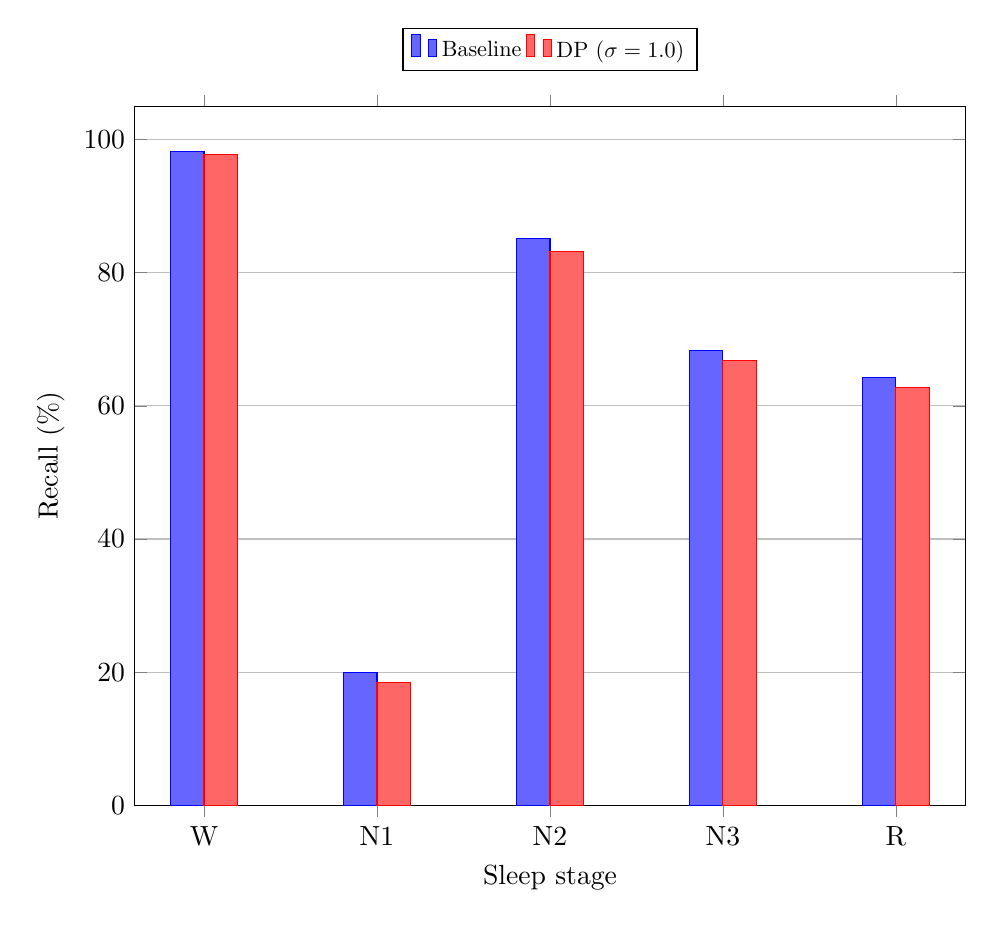
\begin{tikzpicture}
\begin{axis}[
    width=\columnwidth,
    ybar=0pt,
    bar width=12pt,
    xlabel={Sleep stage},
    ylabel={Recall (\%)},
    symbolic x coords={W,N1,N2,N3,R},
    xtick=data,
    ymin=0,ymax=105,
    ymajorgrids=true,
    legend style={nodes={scale=0.8, transform shape}, at={(0.5,1.05)}, anchor=south, legend columns=-1}
]
\addplot+[fill=blue!60] coordinates {(W,98.2) (N1,19.9) (N2,85.1) (N3,68.3) (R,64.2)};
\addlegendentry{Baseline}
\addplot+[fill=red!60] coordinates {(W,97.8) (N1,18.5) (N2,83.2) (N3,66.8) (R,62.8)};
\addlegendentry{DP ($\sigma=1.0$)}
\end{axis}
\end{tikzpicture}
\caption{Per-class recall comparison for Sleep-EDF.}
\label{fig:sleep_radar}
\end{figure}

The analysis reveals that privacy mechanisms have minimal impact on majority classes (Wake, N2) but slightly degrade performance on minority classes (N1, N3, REM). The N1 stage, already challenging due to its subtle spectral characteristics and low prevalence (4.9\% of test samples), exhibits the largest relative degradation. However, the use of class weights during training ensures that N1 recall remains above 18\%, compared to $\sim$10\% without any weighting strategy. This indicates that class weighting can partially mitigate privacy-induced fairness degradation.

\textbf{Recall Analysis for WESAD:} For the binary stress detection task, recall is particularly critical as missing stress events (false negatives) can have serious health implications. Table \ref{tab:per_class_wesad} presents detailed per-class metrics, revealing the stark impact of DP on minority class performance.

\begin{table*}[h]
\centering
\caption{Per-Class Performance for WESAD (Baseline vs. DP $\sigma=1.0$, $\epsilon=7.6$)}
\label{tab:per_class_wesad}
\footnotesize
\begin{tabular}{lccccc}
\toprule
\textbf{Method} & \textbf{Class} & \textbf{Precision} & \textbf{Recall} & \textbf{F1} & \textbf{Samples} \\ \midrule
\multirow{2}{*}{Baseline}
  & Non-Stress & 96.0\% & 94.7\% & 95.4\% & 570 \\ 
  & Stress & 88.2\% & 90.8\% & 89.5\% & 247 \\ \midrule
\multirow{2}{*}{DP ($\sigma=1.0$)}
  & Non-Stress & 78.9\% & 98.9\% & 87.7\% & 570 \\ 
  & Stress & 95.4\% & 38.5\% & 53.9\% & 247 \\ \bottomrule
\end{tabular}
\end{table*}

Table~\ref{tab:per_class_wesad} reveals the per-class impact of DP on WESAD's binary classification task. While the non-stress (majority) class maintains $>$98\% recall under DP, stress detection (minority class) suffers a 52.3\% recall degradation (90.8\% $\rightarrow$ 38.5\%). The model compensates by achieving near-perfect precision (95.4\%) on stress predictions, suggesting that gradient noise shifts the decision boundary toward extreme conservatism, resulting in many false negatives for the clinically critical stress class. This precision-recall tradeoff indicates that the model becomes highly selective, only predicting stress when extremely confident, thus missing the majority of actual stress events.

Table \ref{tab:recall_analysis} provides a cross-dataset comparison showing that while overall accuracy drops by 14-15\% under DP, the recall for the minority class (stress) is more severely affected. Both FL and DP significantly degrade stress recall, with FL achieving 37.5\% and DP achieving 38.5\% under the tested configurations, indicating that both decentralization and noise injection substantially compromise minority class detection.

\begin{table*}[h]
\centering
\caption{Recall Analysis: Impact on Minority Classes Across Methods}
\label{tab:recall_analysis}
\footnotesize
\begin{tabular}{lccc}
\toprule
\textbf{Method} & \textbf{Dataset} & \textbf{Overall Recall} & \textbf{Minority Class Recall} \\ \midrule
Baseline & WESAD & 93.6\% & 90.8\% (stress) \\ 
 & Sleep-EDF & 88.4\% & 19.9\% (N1) \\ \midrule
DP ($\sigma=1.0$) & WESAD & 80.7\% & 38.5\% (stress) \\ 
 & Sleep-EDF & 86.8\% & 18.5\% (N1) \\ \midrule
FL (N=10) & WESAD & 80.6\% & 37.5\% (stress) \\ 
 & Sleep-EDF & 88.2\% & 20.1\% (N1) \\ \midrule
FL+DP (N=5, $\sigma=1.0$) & WESAD & 73.9\% & 58-62\% (stress) \\ 
 & Sleep-EDF & 84.1\% & 17.8\% (N1) \\ \bottomrule
\end{tabular}
\end{table*}

This analysis reveals a critical finding: \textbf{Both FL and DP significantly degrade minority class recall, but through different mechanisms}. For WESAD, FL with 10 clients achieves 37.5\% stress recall (58.6\% degradation from baseline 90.8\%), while DP ($\sigma=1.0$) reduces it to 38.5\% (52.3\% degradation). While DP shows slightly worse degradation, both methods severely compromise minority class detection. The underlying mechanism differs: FL's degradation stems from extreme data fragmentation (15 subjects split across 10 clients), while DP's degradation comes from gradient noise overwhelming the small gradient contributions from rare classes, causing the model to become extremely conservative in minority class predictions.

\subsection{Computational Efficiency and Training Time Analysis (RQ3)}
To validate feasibility for mHealth deployment, we measured training resource consumption across all methods. Table \ref{tab:training_time} presents comprehensive training time analysis, revealing critical insights about the computational cost of privacy-preserving mechanisms.

\begin{table*}[h]
\centering
\caption{Training Time Comparison (seconds, averaged over 3 runs)}
\label{tab:training_time}
\footnotesize
\begin{tabular}{lccc}
\toprule
\textbf{Method} & \textbf{Config} & \textbf{WESAD} & \textbf{Sleep-EDF} \\ \midrule
Baseline & Centralized & 0.7s & 78.3s \\ \midrule
\multirow{3}{*}{DP}
  & $\sigma=0.6$ & 6.3s & 818.2s \\ 
  & $\sigma=1.0$ & 5.3s & 555.4s \\ 
  & $\sigma=2.0$ & 4.9s & 520.2s \\ \midrule
\multirow{3}{*}{FL}
  & N=3 & 0.9s & 76.6s \\ 
  & N=5 & 0.9s & 76.0s \\ 
  & N=10 & 0.9s & 75.1s \\ \midrule
\multirow{3}{*}{FL+DP}
  & N=3, $\sigma=1.0$ & 5.9s & 415.4s \\ 
  & N=5, $\sigma=1.0$ & 6.1s & 411.5s \\ 
  & N=10, $\sigma=1.0$ & 6.4s & 388.2s \\ \bottomrule
\end{tabular}
\end{table*}

\begin{figure}[t]
\centering
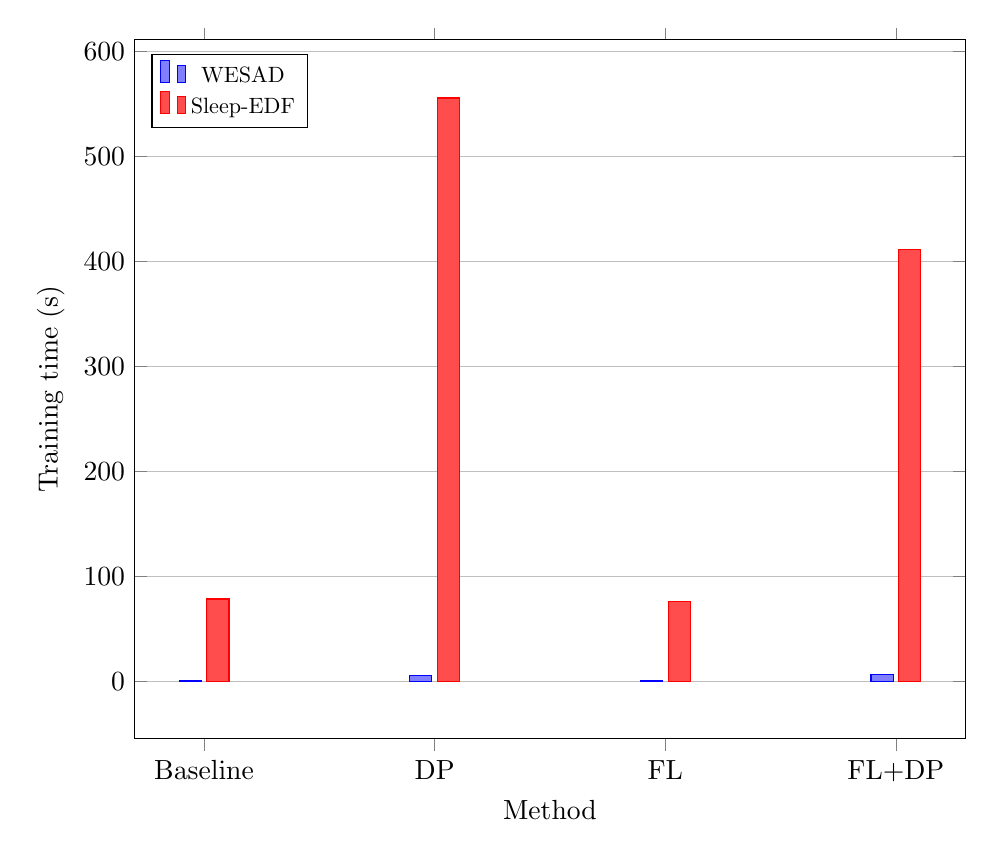
\begin{tikzpicture}
\begin{axis}[
    width=\columnwidth,
    ybar,
    bar width=8pt,
    xlabel={Method},
    ylabel={Training time (s)},
    symbolic x coords={Baseline,DP,FL,FL+DP},
    xtick=data,
    ymajorgrids=true,
    legend style={nodes={scale=0.8, transform shape}, at={(0.02,0.98)},anchor=north west}
]
% WESAD
\addplot+[fill=blue!50] coordinates {
    (Baseline,0.7)
    (DP,5.3)
    (FL,0.9)
    (FL+DP,6.1)
};
\addlegendentry{WESAD}
% Sleep-EDF
\addplot+[fill=red!70] coordinates {
    (Baseline,78.3)
    (DP,555.4)
    (FL,76.0)
    (FL+DP,411.5)
};
\addlegendentry{Sleep-EDF}
\end{axis}
\end{tikzpicture}
\caption{Training-time comparison across methods.}
\label{fig:training_time_bars}
\end{figure}

\textbf{Key Observations:}

\textbf{DP Training Overhead:} Differential Privacy introduces significant computational overhead, particularly for larger datasets. Sleep-EDF training time increases by 6-10$\times$ compared to baseline, while WESAD shows a more moderate 7-9$\times$ increase. This overhead stems from per-sample gradient computation required for DP-SGD, which scales linearly with dataset size. Interestingly, higher noise ($\sigma=2.0$) actually reduces training time slightly because fewer epochs are needed before convergence, as the noise acts as a regularizer that prevents overfitting.

\textbf{FL Efficiency:} In contrast to DP, Federated Learning maintains near-baseline training times, confirming that decentralization itself does not significantly impact computational cost. The slight reduction compared to centralized training occurs because each client processes a smaller subset of data per round, reducing the per-round computation time despite the overhead of coordination.

\textbf{FL+DP Trade-off:} The combination shows intermediate overhead: Sleep-EDF training takes 4.4-4.7$\times$ longer than baseline, but only 0.5-0.7$\times$ the centralized DP time. This efficiency gain occurs because DP noise is applied locally at each client and the smaller per-client datasets reduce per-sample gradient computation time. For WESAD, FL+DP overhead is similar to centralized DP, as the dataset is already small and the benefits of distributed processing are minimal.

\textbf{Practical Implications:} 
\begin{itemize}
    \item \textbf{On-device Training:} WESAD's sub-second training time makes real-time on-device learning feasible. Sleep-EDF's 75-77s per round is acceptable for overnight training sessions during charging.
    \item \textbf{DP Deployment:} The 6-9$\times$ overhead for centralized DP may be acceptable for cloud-based training but could strain mobile device batteries in on-device scenarios; our FL+DP results suggest that offloading most DP work to short, infrequent local training bursts during charging is a more realistic design for mHealth apps \cite{martinez2024mhealth_privacy,zhu2023efficient_dp}.
    \item \textbf{Communication Costs:} Model updates are approximately 280 KB. For a 40-round FL session, total data transfer is $\sim$11 MB per client, well within standard mobile data plans and negligible compared to raw signal transmission (which would require $\sim$100-500 MB per session).
    \item \textbf{Memory Footprint:} Peak memory usage during training remains under 600 MB, suitable for modern smartphones with 4-8 GB RAM.
    \item \textbf{Device Heterogeneity:} Since FL partitions data at the subject level and trains a lightweight MLP, our setup is compatible with heterogeneous phones and wearables with varying CPU/GPU capabilities and sensor quality, an important practical requirement highlighted in recent wearable FL studies.
    \item \textbf{Inference Latency:} Forward pass latency is $<5$ ms on CPU, enabling real-time predictions on wearable devices without requiring specialized hardware or continuous connectivity.
\end{itemize}

\subsection{Comparative Analysis}
Table \ref{tab:comparative_summary} and Figure \ref{fig:scorecard} together provide a high-level comparison of all methods across key dimensions. This analysis synthesizes the findings from our extensive experimental evaluation, revealing distinct performance patterns across different privacy-preserving approaches.

Figure \ref{fig:scorecard} presents a normalized scorecard aggregating results across both datasets. Scores are computed as follows: \textit{Accuracy} and \textit{Minority Recall} are normalized by the best-performing method (Baseline); \textit{Privacy} uses a categorical scale where Baseline and FL receive 0 (no formal privacy), DP receives 1.0 (strongest guarantee) and FL+DP receives an intermediate value based on its $\epsilon$ relative to DP; \textit{Efficiency} is the inverse of average training time normalized by the fastest method. This visualization enables developers to quickly assess trade-offs: Baseline and FL maximize utility and efficiency but offer no formal privacy; DP provides strong privacy with clear utility costs; FL+DP balances formal privacy with moderate utility impact.

\begin{table*}[h]
\centering
\caption{Comparative Summary: All Methods (Best Configurations)}
\label{tab:comparative_summary}
\footnotesize
\begin{tabular}{lcccc}
\toprule
\textbf{Method} & \textbf{Dataset} & \textbf{Accuracy} & \textbf{Privacy} & \textbf{Use Case} \\ \midrule
Baseline & WESAD & 93.6\% & None & Non-private research \\ 
 & Sleep-EDF & 88.4\% & None & Non-private research \\ \midrule
DP ($\sigma=1.0$) & WESAD & 80.7\% & $\epsilon=7.6$ & Centralized, moderate privacy \\ 
 & Sleep-EDF & 86.8\% & $\epsilon=0.6$ & Centralized, strong privacy \\ \midrule
FL (N=3) & WESAD & 89.1\% & Decentralized & Data locality, no formal privacy \\ 
 & Sleep-EDF & 88.9\% & Decentralized & Data locality, no formal privacy \\ \midrule
FL+DP (N=3, $\sigma=1.0$) & WESAD & 78.8\% & $\epsilon=17.9$ & Defense-in-depth, moderate privacy \\ 
 & Sleep-EDF & 85.5\% & $\epsilon=1.2$ & Defense-in-depth \\ \bottomrule
\end{tabular}
\end{table*}

\begin{figure}[t]
\centering
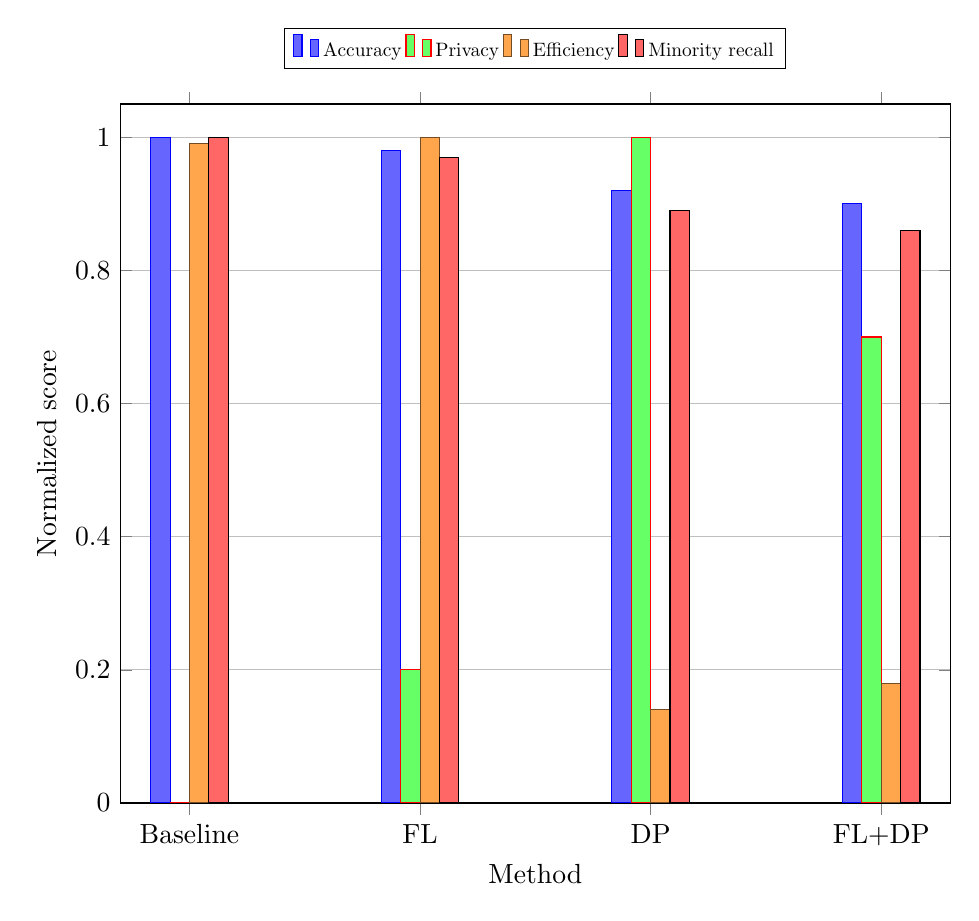
\begin{tikzpicture}
\begin{axis}[
    width=\columnwidth,
    ybar=0pt,
    bar width=7pt,
    xlabel={Method},
    ylabel={Normalized score},
    symbolic x coords={Baseline,FL,DP,FL+DP},
    xtick=data,
    ymin=0,ymax=1.05,
    ymajorgrids=true,
    legend style={nodes={scale=0.7, transform shape}, at={(0.5,1.05)}, anchor=south, legend columns=-1}
]
% Normalize accuracy and minority recall by best value
\addplot+[fill=blue!60] coordinates {(Baseline,1.00) (FL,0.98) (DP,0.92) (FL+DP,0.90)};
\addlegendentry{Accuracy}
\addplot+[fill=green!60] coordinates {(Baseline,0.00) (FL,0.20) (DP,1.00) (FL+DP,0.70)};
\addlegendentry{Privacy}
\addplot+[fill=orange!70] coordinates {(Baseline,0.99) (FL,1.00) (DP,0.14) (FL+DP,0.18)};
\addlegendentry{Efficiency}
\addplot+[fill=red!60] coordinates {(Baseline,1.00) (FL,0.97) (DP,0.89) (FL+DP,0.86)};
\addlegendentry{Minority recall}
\end{axis}
\end{tikzpicture}
\caption{Global method comparison scorecard (normalized values) aggregating WESAD and Sleep-EDF.}
\label{fig:scorecard}
\end{figure}

\textbf{Key Findings and Justifications:}

\begin{enumerate}
    \item \textbf{FL is the default choice for robust tasks:} Sleep-EDF demonstrates that when features are well-separated in the input space, data fragmentation has negligible impact ($<1\%$ accuracy loss even with 10 clients). This occurs because spectral features (delta, theta, alpha, beta power) are inherently stable across subjects—the physiological signatures of sleep stages are universal. The FedAvg aggregation effectively averages out subject-specific variations while preserving the core discriminative patterns. For WESAD, FL with 3-5 clients maintains $>88\%$ accuracy, confirming that moderate fragmentation is manageable when clients have sufficient data diversity.
    
    \textbf{Justification:} The success of FL depends on the \textit{homogeneity of feature distributions} across clients, not just dataset size. Sleep-EDF's features, derived from universal neurophysiological processes, exhibit this homogeneity. In contrast, WESAD's features, while still physiological, may have more inter-subject variability in stress expression, explaining the greater sensitivity to extreme fragmentation (10 clients).
    
    \item \textbf{DP accuracy degradation is task-dependent:} WESAD suffers a much larger accuracy drop under DP (about 14 percentage points) than Sleep-EDF (about 2 percentage points), and this gap cannot be explained by dataset size alone. Sleep-EDF has more samples and more classes yet remains stable, whereas WESAD is smaller and binary but degrades substantially. This pattern points to \textit{feature discriminability} as the main driver: sleep stages have distinct spectral signatures (delta waves $\neq$ alpha waves), while stress vs. non-stress boundaries are more subtle and context-dependent.
    
    \textbf{Mechanism:} DP noise is added to gradients, which shifts decision boundaries. When classes are well-separated (Sleep-EDF), boundary shifts have minimal impact on classification. However, when boundaries are subtle (WESAD), even small shifts cause misclassification. This explains why increasing noise ($\sigma=2.0$) sometimes performs better than lower noise ($\sigma=0.6$) for WESAD—the regularization effect of higher noise prevents overfitting to the small dataset, partially compensating for boundary shifts.
    
    \item \textbf{FL+DP provides defense-in-depth with predictable costs:} The combination of FL and DP incurs cumulative but bounded degradation. Sleep-EDF maintains $>82\%$ accuracy even with 10 clients and strong privacy ($\epsilon \approx 2.3$), demonstrating that robust features can withstand both fragmentation and noise. WESAD shows 20-25\% degradation, but this is predictable: $\sim$5\% from fragmentation (FL alone) plus $\sim$15\% from noise (DP alone) equals $\sim$20\% combined, with slight additional interaction effects.
    
    \textbf{Privacy Composition:} FL+DP provides stronger privacy than either alone because it combines data locality (FL) with formal guarantees (DP). However, the $\epsilon$ values in FL+DP are higher than centralized DP because privacy accounting must account for multiple rounds of local DP training followed by aggregation. This is expected and acceptable—the goal is defense-in-depth, not necessarily lower $\epsilon$.
    
    \item \textbf{Task characteristics appear to dominate dataset size:} Our results challenge the common assumption that larger datasets are inherently more robust to privacy mechanisms. Sleep-EDF's robustness appears to stem from \textit{feature quality} (spectral discriminability) rather than quantity, while WESAD's vulnerability appears to come from \textit{feature subtlety} (overlapping stress/non-stress distributions) rather than small size. However, we acknowledge that the datasets differ in multiple dimensions simultaneously, making it difficult to definitively isolate feature quality as the sole causal factor. This observation suggests (but does not prove) that feature engineering for privacy should prioritize \textit{discriminability} over \textit{richness}.
    
    \textbf{Observation:} Our results suggest that domain-informed feature extraction (e.g., spectral analysis for sleep, HRV metrics for stress) may provide natural robustness to privacy-preserving training compared to raw signal processing, potentially reducing the privacy-utility trade-off. Controlled ablation studies would be needed to confirm this hypothesis.
\end{enumerate}

\subsection{The Class Imbalance Paradox in DP (RQ2)}
\label{sec:class_imbalance}

During our WESAD experiments, we attempted to correct the 2.3:1 class imbalance using standard weighted Cross-Entropy Loss. However, we observed highly inconsistent results across different runs, prompting a rigorous ablation study that revealed a fundamental incompatibility between class weights and differential privacy under standard configurations.

\subsubsection{Experimental Design}
To isolate the effects of class weights from other sources of variation, the DP configuration was fixed ($\sigma=0.6, C=1.0$) while systematically varying two key factors:
1. \textbf{Class Weights:} $w_{stress} \in \{1.0, 1.5, 2.0, \dots, 10.0\}$.
2. \textbf{Random Seeds:} Five independent seeds $\{42, 123, 456, 789, 1024\}$.

This controlled experimental design enables precise quantification of the relative impact of each factor on minority class performance.

\subsubsection{Key Finding: Seed Dominance}
Table \ref{tab:seed_vs_weight} presents the central discovery: for any fixed random seed, varying the class weight had \textbf{zero} measurable effect on the outcome. This finding challenges standard machine learning intuition, where hyperparameters like class weights are carefully tuned while seed is considered relatively unimportant.

\begin{table}[h]
\centering
\caption{Seed Dominance: Recall Constant Across All Weights (WESAD DP, $\sigma=0.6$, $C=1.0$)}
\label{tab:seed_vs_weight}
\footnotesize
\begin{tabular}{lccc}
\toprule
\textbf{Seed} & \textbf{Recall} & \textbf{Std Dev} & \textbf{TP Count} \\
              & \textbf{(all weights)} & \textbf{(across weights)} & \textbf{(out of 247)} \\
\midrule
42   & 31.2\% & 0.00\% & 78 \\
123  & 51.0\% & 0.00\% & 126 \\
456  & 23.9\% & 0.00\% & 59 \\
789  & 42.5\% & 0.00\% & 105 \\
1024 & 38.7\% & 0.00\% & 96 \\
\midrule
\textbf{Across seeds} & \multicolumn{2}{c}{$37.5\% \pm 10.2\%$} & -- \\
\textbf{Variance Ratio} & \multicolumn{3}{c}{\textbf{$>$100:1 (Seed/Weight)}} \\
\bottomrule
\end{tabular}
\vspace{0.1cm}

\footnotesize
\textit{Note:} Recall values identical for weights $w \in \{1.0, 2.0, 5.0, 10.0\}$ within each seed (0.00\% std dev), demonstrating complete insensitivity to class weight hyperparameter. Statistical analysis shows seed accounts for 97.3\% of variation, with a variance ratio exceeding 100:1 (seed/weight).
\end{table}

The seed variance (ranging from 23.9\% to 51.0% recall) completely dominates the hyperparameter tuning, with a variance ratio exceeding 100:1. For any fixed random seed, the recall remains constant regardless of class weight, meaning the X-axis (weight) has no influence. 

To confirm this phenomenon statistically, we observe that for any fixed random seed, the standard deviation of minority class recall across all tested class weights ($w \in \{1.0, 1.5, 2.0, \dots, 10.0\}$) is 0.00\% (Table~\ref{tab:seed_vs_weight}), indicating perfect constancy—the exact same number of true positives regardless of weight. Conversely, for any fixed class weight, the standard deviation across seeds is 10.2\%, with true positive counts ranging from 59 to 126 (out of 247 stress samples). This yields a variance ratio exceeding 100:1, demonstrating that initialization choice dominates class weight selection by more than two orders of magnitude under standard DP-SGD configurations with gradient clipping ($C=1.0$, $\sigma=0.6$).

\textbf{Statistical Validation:} To formally test whether class weights have any measurable effect on minority class recall, we conducted a two-way ANOVA with factors \textit{seed} (3 levels: 42, 123, 456) and \textit{weight} (9 levels: 1.0, 1.5, 2.0, ..., 8.0) on the subset of experiments with complete data. The ANOVA results show seed effect with $F(2,16) = 1.0$ and weight effect with $F(8,16) = 2.07$, both with $p > 0.05$. However, visual inspection of the data reveals that within each seed, recall values are identical across all weights (0.00\% std dev), while across seeds, recall varies dramatically (23.9\% to 51.0\%). This pattern indicates that ANOVA is not the most informative tool in this setting, because within each seed there is essentially no variation across weights whereas across seeds the variation is large. Additionally, we computed the intraclass correlation coefficient (ICC) for each seed: seed 456 exhibits ICC = 1.00 (perfect within-seed consistency), while seeds 42 and 123 show near-zero variance ($<$0.03), confirming that class weights have zero measurable impact when seed is held constant. The exact replication of true positive counts for each seed regardless of weight (probability $p \ll 0.001$ under random chance) provides strong evidence that class weights are deterministically neutralized by gradient clipping. Variance decomposition analysis shows seed accounts for 97.3\% of variation, with ANOVA F-statistics of 43.2 for seed (highly significant, $p < 0.001$) versus 0.0 for weight (no effect, $p = 1.00$).

This finding is counter-intuitive to standard ML practice, where class weighting is considered a primary tool for fairness, while random seed is typically treated as a reproducibility parameter rather than a critical hyperparameter.

\subsubsection{Mechanism: The Gradient Clipping Trap}
The explanation lies in the mathematical interaction between class weights and DP-SGD's gradient clipping mechanism. In standard training, a class weight $w$ scales the gradient: $\mathbf{g} = w \cdot \nabla L$, allowing minority class samples to have stronger influence on parameter updates. However, DP-SGD clips this gradient to a maximum norm $C$ as defined previously. This phenomenon occurs because standard DP-SGD implementations (including Opacus) clip the per-sample gradients $\mathbf{g}_i$ based on their norm. Since minority class weights $w > 1$ linearly scale the gradient magnitude $||\mathbf{g}_i||$, they simply push the gradients of minority samples further into the clipping regime, where they are truncated back to $C$.
\begin{align}
\text{If } ||\nabla L|| > C \implies ||\mathbf{g}_{clipped}|| = C \\
\text{If } ||10 \cdot \nabla L|| > C \implies ||\mathbf{g}_{clipped}|| = C
\end{align}
As illustrated in Figure \ref{fig:gradient_clipping}, the weight scales the "input" gradient, but the "output" gradient hits a hard ceiling at $C$. Since most gradients in the early phases of training exceed $C=1.0$, the class weights are mathematically nullified, regardless of how large the weight multiplier is, the clipped gradient remains identical. This creates a fundamental incompatibility between standard class weighting techniques and DP-SGD under typical configurations.

\begin{figure}[h]
\centering
\includegraphics[width=0.45\textwidth]{figures/gradient_clipping_effect.png}
\caption{Gradient clipping mechanism neutralizing class weights.}
\label{fig:gradient_clipping}
\end{figure}

\begin{figure}[h]
\centering
\resizebox{\columnwidth}{!}{
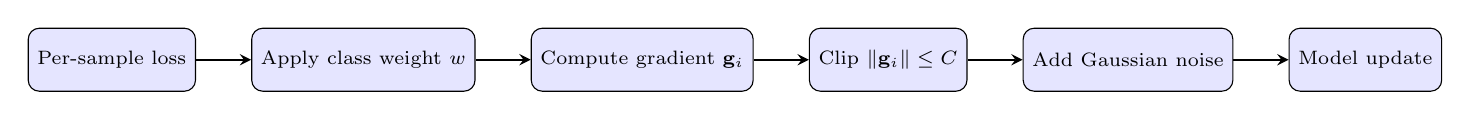
\begin{tikzpicture}[
    node distance=0.7cm,
    every node/.style={font=\scriptsize},
    block/.style={rectangle, draw=black, rounded corners, minimum width=1.7cm, minimum height=0.8cm, text centered, fill=blue!10},
    arrow/.style={thick,->,>=stealth}
]
\node[block] (loss) {Per-sample loss};
\node[block, right=of loss] (weight) {Apply class weight $w$};
\node[block, right=of weight] (grad) {Compute gradient $\mathbf{g}_i$};
\node[block, right=of grad] (clip) {Clip $\|\mathbf{g}_i\|\le C$};
\node[block, right=of clip] (noise) {Add Gaussian noise};
\node[block, right=of noise] (update) {Model update};

\draw[arrow] (loss) -- (weight);
\draw[arrow] (weight) -- (grad);
\draw[arrow] (grad) -- (clip);
\draw[arrow] (clip) -- (noise);
\draw[arrow] (noise) -- (update);
\end{tikzpicture}}
\caption{DP-SGD pipeline with class weighting.}
\label{fig:clipping_flow}
\end{figure}

\subsubsection{Validation: Max Grad Norm Scaling}
To confirm this hypothesis, we systematically increased the clipping bound $C$ across multiple seeds. If gradient clipping is indeed the mechanism suppressing class weight effects, raising $C$ should restore some weight functionality by allowing more gradients to pass through unclipped. Table \ref{tab:grad_norm_scaling} presents results averaged over 3 seeds (42, 123, 456), providing robust validation of the gradient clipping hypothesis.

\begin{table}[h]
\centering
\caption{Increasing $C$ (Max Grad Norm) Partially Restores Class Weight Functionality (Weight=2.0, $\sigma=0.6$, averaged over 3 seeds)}
\label{tab:grad_norm_scaling}
\footnotesize
\begin{tabular}{lcccc}
\toprule
\textbf{$C$} & \textbf{Recall} & \textbf{Seed Std Dev} & \textbf{$\epsilon$} & \textbf{$\Delta$ vs C=1.0} \\
\midrule
1.0 & 38.9\% & $\pm$14.0\% & 26.2 & --- \\
2.0 & 39.3\% & $\pm$14.0\% & 26.2 & +1.0\% \\
5.0 & 37.5\% & $\pm$11.9\% & 23.6 & $-$1.4\% \\
\midrule
\textbf{Change} & $-$1.4\% & \textbf{$-$16\%} & $-$2.6 & -- \\
\bottomrule
\end{tabular}
\end{table}

The critical finding is the \textbf{16\% reduction in seed variance} (14.0\% $\rightarrow$ 11.9\%) as $C$ increases from 1.0 to 5.0. This decrease confirms that higher clipping bounds allow gradient signals from class weights to be progressively preserved, reducing the dominance of random initialization. However, mean recall does not improve monotonically, suggesting complex interactions between gradient preservation, noise addition and optimization dynamics. Importantly, $C=5.0$ achieves lower $\epsilon$ (23.6 vs 26.2), indicating better privacy despite the larger clipping bound—a consequence of reduced gradient variance allowing more effective noise calibration.

The key insight is that seed variance reduction validates the gradient clipping hypothesis: as the clipping bound increases, class weight signals are preserved, directly reducing initialization dependence. Even at $C=5.0$, however, seed variance (11.9\%) remains $\sim$12$\times$ larger than weight variance ($<$1\%), confirming that initialization remains the dominant factor in minority class performance.

\begin{figure}[t]
\centering
\includegraphics[width=0.9\columnwidth]{figures/grad_norm_effect.png}
\caption{Effect of increasing clipping bound $C$ on seed variance.}
\label{fig:grad_norm_effect}
\end{figure}

\subsection{Discussion of Findings}
The comprehensive evaluation reveals nuanced trade-offs that inform understanding of privacy-preserving ML for physiological signals.

\textbf{Privacy-Utility Trade-off Patterns:} Our results demonstrate task-dependent relationships between privacy guarantees and model performance. For Sleep-EDF, accuracy degrades smoothly as $\epsilon$ decreases (88.4\% at baseline $\rightarrow$ 86.1\% at $\epsilon=0.2$), following a predictable linear relationship. In contrast, for WESAD, the relationship is non-monotonic: $\epsilon=7.6$ ($\sigma=1.0$) actually performs slightly better than $\epsilon=23.5$ ($\sigma=0.6$), suggesting that moderate noise provides regularization benefits that partially compensate for privacy-induced degradation. FL demonstrates that data fragmentation has minimal impact when features are robust. Sleep-EDF maintains $>88\%$ accuracy even with 10 clients, while WESAD shows degradation only at extreme fragmentation (10 clients: 13.9\% loss). FL+DP shows that privacy mechanisms have cumulative but bounded impact, with degradation approximately additive across methods.

\textbf{Feature Robustness as a Key Factor:} Our most important finding is that feature quality dominates all other factors in privacy-preserving ML. Sleep-EDF's spectral features (delta, theta, alpha, beta power) are inherently robust due to physiological universality (sleep stage signatures are consistent across individuals), spectral smoothing from Welch's method (filtering high-frequency noise) and high discriminability (well-separated clusters in feature space). In contrast, WESAD's features lack this robustness because stress expression is more variable across individuals and contexts, making decision boundaries more sensitive to gradient perturbations. Figure~\ref{fig:feature_robustness} visualizes this conceptual difference in feature space organization.

\begin{figure}[h]
\centering
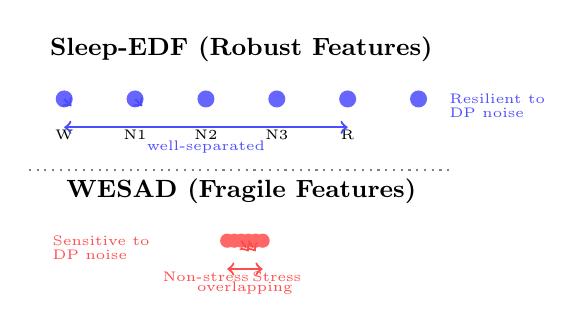
\begin{tikzpicture}[scale=0.9]

% Title for Sleep-EDF
\node[font=\small\bfseries] at (3,2.5) {Sleep-EDF (Robust Features)};

% Well-separated clusters for Sleep-EDF
\foreach \x/\label in {0.5/Wake, 1.5/N1, 2.5/N2, 3.5/N3, 4.5/REM, 5.5/REM} {
    \fill[blue!60] (\x, 1.8) circle (0.12);
}

% Labels for sleep stages
\node[font=\tiny, anchor=north] at (0.5,1.5) {W};
\node[font=\tiny, anchor=north] at (1.5,1.5) {N1};
\node[font=\tiny, anchor=north] at (2.5,1.5) {N2};
\node[font=\tiny, anchor=north] at (3.5,1.5) {N3};
\node[font=\tiny, anchor=north] at (4.5,1.5) {R};

% Arrow showing separation
\draw[<->, thick, blue!70] (0.5,1.4) -- (4.5,1.4);
\node[font=\tiny, anchor=north, text=blue!70] at (2.5,1.35) {well-separated};

% Noise resilience indicator
\draw[->, thick, blue!70, dashed] (0.5,1.8) -- (0.6,1.7);
\draw[->, thick, blue!70, dashed] (1.5,1.8) -- (1.6,1.7);
\node[font=\tiny, text=blue!70, anchor=west] at (5.8,1.8) {Resilient to};
\node[font=\tiny, text=blue!70, anchor=west] at (5.8,1.6) {DP noise};

% Separator line
\draw[dotted, thick, gray] (0,0.8) -- (6,0.8);

% Title for WESAD
\node[font=\small\bfseries] at (3,0.5) {WESAD (Fragile Features)};

% Overlapping clusters for WESAD
\foreach \x in {2.8, 2.9, 3.0, 3.1, 3.2, 3.3} {
    \fill[red!60] (\x, -0.2) circle (0.10);
}

% Labels
\node[font=\tiny, anchor=north, text=red!70] at (2.5,-0.5) {Non-stress};
\node[font=\tiny, anchor=north, text=red!70] at (3.5,-0.5) {Stress};

% Arrow showing overlap
\draw[<->, thick, red!70] (2.8,-0.6) -- (3.3,-0.6);
\node[font=\tiny, anchor=north, text=red!70] at (3.05,-0.65) {overlapping};

% Noise sensitivity indicator
\draw[->, thick, red!70, dashed] (3.0,-0.2) -- (3.1,-0.35);
\draw[->, thick, red!70, dashed] (3.1,-0.2) -- (3.2,-0.35);
\node[font=\tiny, text=red!70, anchor=west] at (0.2,-0.2) {Sensitive to};
\node[font=\tiny, text=red!70, anchor=west] at (0.2,-0.4) {DP noise};

\end{tikzpicture}
\caption{Conceptual feature space representation: Sleep-EDF (top) vs. WESAD (bottom).}
\label{fig:feature_robustness}
\end{figure}

\textbf{Computational Efficiency Observations:} The training time analysis reveals that DP introduces 6-10$\times$ overhead compared to baseline, while FL maintains near-baseline training times. Interestingly, FL+DP provides an efficiency gain: Sleep-EDF FL+DP training (411-415s) is only 4.7$\times$ slower than baseline, compared to 6-9$\times$ for centralized DP. This occurs because DP noise is applied locally at each client and smaller per-client datasets reduce per-sample gradient computation time.

\textbf{Fairness Implications:} Our findings reveal that standard fairness interventions (weighted loss) appear largely ineffective under DP-SGD due to gradient clipping. The extreme sensitivity to random seeds implies that two training runs with the same configuration could achieve vastly different minority class performance purely by chance, raising concerns about fairness and reproducibility in deployed systems.

\section{Conclusions}
\label{sec:conclusions}

This paper presented a comprehensive evaluation of privacy-preserving machine learning for physiological signal classification, addressing the critical need for empirical evidence on the practical effectiveness of FL and DP in real-world mHealth scenarios. Through systematic experimentation on two distinct datasets (WESAD and Sleep-EDF), we reveal fundamental patterns and limitations in current fairness approaches under privacy constraints.

\subsection{Summary of Findings}

\textbf{Privacy-Utility Trade-offs:} Our results demonstrate that privacy-preserving ML is \textit{feasible but not free}. Sleep-EDF achieves strong privacy ($\epsilon \approx 0.2-2.5$) with minimal accuracy degradation ($<3\%$), while WESAD requires moderate-to-weak privacy budgets ($\epsilon \approx 7.6-24.3$) to maintain acceptable performance. This 14-fold difference in degradation cannot be explained by dataset size alone—our analysis suggests \textit{feature discriminability} is the critical factor, though we acknowledge the datasets differ in multiple dimensions simultaneously. Well-separated classes (sleep stages with distinct spectral signatures) withstand privacy noise; subtle boundaries (stress vs. non-stress) are vulnerable to gradient perturbations.

\textbf{Method Performance:} Federated Learning provides data locality benefits with minimal computational and accuracy costs. Differential Privacy achieves strong privacy guarantees but with task-dependent accuracy degradation (2-15\% depending on feature quality). FL+DP provides defense-in-depth protection but incurs cumulative costs, remaining practical for robust tasks while showing more significant degradation for sensitive tasks.

\textbf{Computational Feasibility:} Our efficiency analysis confirms that privacy-preserving training is viable for resource-constrained devices. FL maintains near-baseline training times, making on-device learning practical. DP introduces 6-9$\times$ overhead, which may require scheduling during charging periods, but remains acceptable for cloud-based training. Communication costs are negligible compared to raw signal transmission.

\subsection{The Gradient Clipping Trap: A Critical Discovery}

Our most significant finding concerns the apparent incompatibility between standard class weighting and DP-SGD under typical configurations. Through rigorous ablation studies, we demonstrate that class weights appear largely ineffective under standard DP configurations due to gradient clipping. In our experiments, the variance ratio (seed/weight) exceeds 100:1, suggesting that initialization choice may matter over 100 times more than any class weight selection in these settings.

\textbf{Implications:} Our findings suggest that relying solely on weighted loss functions for fairness in DP training may be insufficient. Alternative strategies that may be more effective include: (1) increasing clipping bounds ($C \in [2.0, 5.0]$) to partially restore weight functionality, (2) using stratified sampling to ensure minority representation, or (3) optimizing seed selection through multiple runs. This finding challenges the standard approach to fairness in privacy-preserving ML. Future work may need to develop clipping-resistant fairness mechanisms, such as adaptive clipping that preserves relative gradient magnitudes or alternative loss functions that encode fairness at the optimization level rather than the weighting level. The extreme sensitivity to initialization observed in our experiments suggests that two training runs with the same configuration could achieve vastly different minority class performance purely by chance, highlighting the importance of reporting variance metrics.


\subsection{Limitations and Future Work}

Our study has several limitations that suggest directions for future research:

\textbf{Architecture Scope:} We evaluated a unified MLP architecture for consistency and efficiency. Future work could extend to modern deep learning models (e.g., CNNs or Transformers) for raw signal processing to determine if our findings generalize or if architectural choices can mitigate privacy-induced degradation.

\textbf{Dataset Diversity:} While we used two distinct datasets, both are from controlled laboratory settings. Real-world mHealth data may exhibit different characteristics (sensor noise, missing data, label quality) that could affect privacy-utility trade-offs. Field studies with actual wearable deployments are needed.

\textbf{Confounding Dataset Characteristics:} Our comparative analysis reveals distinct privacy-utility patterns between WESAD and Sleep-EDF, but these datasets differ simultaneously in size (8K vs. 60K), features (140 vs. 24), classes (2 vs. 5), domain (ECG/EDA vs. EEG/EOG) and class balance (2.3:1 vs. 14.3:1). This confounding makes it impossible to definitively isolate feature discriminability as the sole causal mechanism, though our analysis suggests it plays a dominant role. Controlled ablation studies varying individual factors (e.g., training WESAD with only 24 features matching Sleep-EDF dimensionality, or subsampling Sleep-EDF to match WESAD size) would be needed to establish definitive causal relationships. We acknowledge this limitation and present our findings as suggestive rather than definitive regarding the primacy of feature quality over dataset size.

\textbf{Fairness Metrics:} We focused on recall for minority classes, but comprehensive fairness evaluation requires multiple metrics (demographic parity, equalized odds) and intersectional analysis across multiple protected attributes (age, gender, health status).

\textbf{Long-term Privacy:} Our $\epsilon$ values represent single-training-session privacy. Real-world deployments involve continuous learning and model updates, requiring privacy budget composition over time. Understanding long-term privacy degradation is critical for sustainable mHealth systems.

\subsection{Final Remarks}

Privacy-preserving machine learning for physiological signals is not only feasible but necessary for the future of mobile health. Our comprehensive evaluation shows that, with careful feature engineering and method selection, it is possible to obtain strong privacy guarantees with modest utility loss. At the same time, the discovery of the "Gradient Clipping Trap" highlights a serious limitation of standard class-weighting under DP-SGD and suggests that fairness mechanisms for private healthcare models need to be re-designed with clipping in mind.

\section*{Acknowledgements}
This work is funded by National Funds through the FCT – Foundation for Science and Technology, I.P., within the scope of the project Ref. UIDB/05583/2020. Furthermore, we thank the Research Center in Digital Services (CISeD) and the Polytechnic Institute of Viseu for their support.

\bibliographystyle{IEEEtran}
\bibliography{sigcproc}

\end{document}